%*******10********20********30********40********50********60********70********80
\clearpage

\subsection{Residual Capabilities after Pure ASR Expansion}

Here the uni-axial compression test result for ASR expanded concrete model is summarised.

As an example, shown in Figure \ref{fig:A30P75_modesl}, compression test for cases with 30\% coarse aggregate, of which 75\% are set to be ASR reactive, will be presented in details.

\begin{figure}[ht!]
\centering
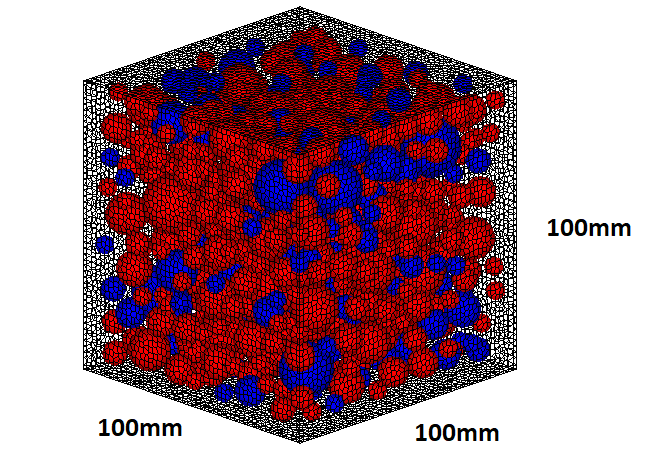
\includegraphics[width=.3\linewidth]{Files/Aggregate/A30P75.png}
  \caption{30\% Coarse Aggregate}
  \label{fig:A30P75_modesl}
\end{figure}

As introduced previously in chapter 2 and chapter 3, one-dimensional global expansion up to 1.3\% has been achieved by giving initial strain step by step at the interfaces between reactive aggregate and paste elements.

After expansion, three-dimensional expanded concrete models are tested under uni-axial compression condition. Displacement of loading boundary is controlled, as the top boundary of the concrete model moves downwards 0.02 mm in each step. Top and bottom boundaries are under fix condition.

In each step of loading, compressive strength in the current step is recorded. As shown in Figure \ref{fig:A30P75FIX_LD}, the Load-Displacement curve obtained here is close to the shape of the normal concrete under fixed boundary compressive test, with increasing strength until reaching the maximum compressive strength, then decreasing until failure happens.

Also, in Figure \ref{fig:A30P75FIX_LD}, the trend of decreasing in maximum compressive strength along with the increasing of one-dimensional global expansion is also shown. With the global expansion increasing up to 1.3\%, the compressive strength reduced gradually to 15.993 MPa, which is 53\% of undamaged model.

The Elastic Modulus, which here calculated as the maximum slope before compressive strength reaching the maximum, also shows the same trend when global expansion increase. While the Elastic Modulus is 33.8 GPa for undamaged model, Elastic Modulus drop to 1.11 GPa when global expansion reached 1.3\%.

Loading with free boundary condition is also simulated here, and presented in Figure \ref{fig:A30P75FREE_LD}. As the boundary are set to be without horizontal frictions, cracks are more easier to open during loading, result in a generally 30\% smaller compressive strength comparing to the result from fixed boundary loading test. This is also corrisbonding with cases in reality. A similar decreasing trend in compressive strength and elastic modulus along with the increase of global expanding ratio can be obtained.

%A30P75FIX

\begin{figure}[ht]
\centering
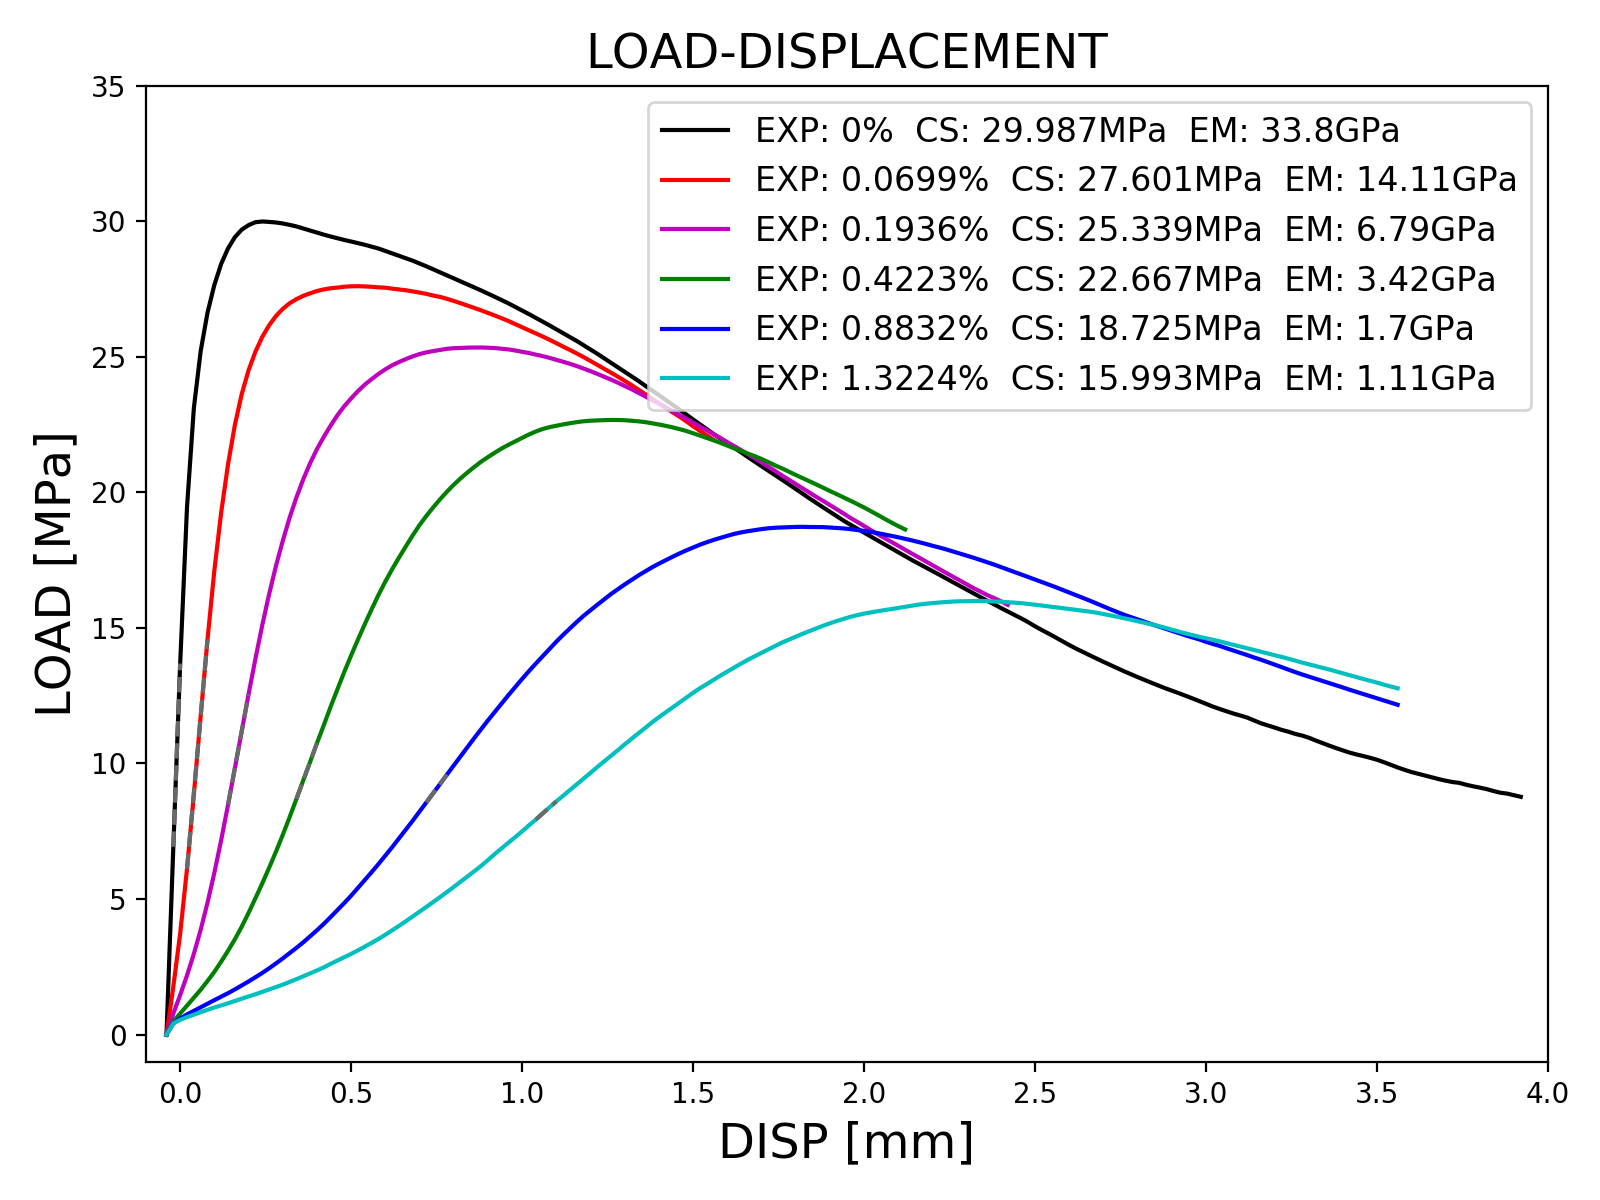
\includegraphics[width=.8\linewidth]{Files/exp_3D/ASR/S13A30P75FIX-LOAD-DISPLACEMENT.png}
  \caption{A30 P75 Fix Load-Displacement}
  \label{fig:A30P75FIX_LD}
\end{figure}

%A30P75FREE

\begin{figure}[ht!]
\centering
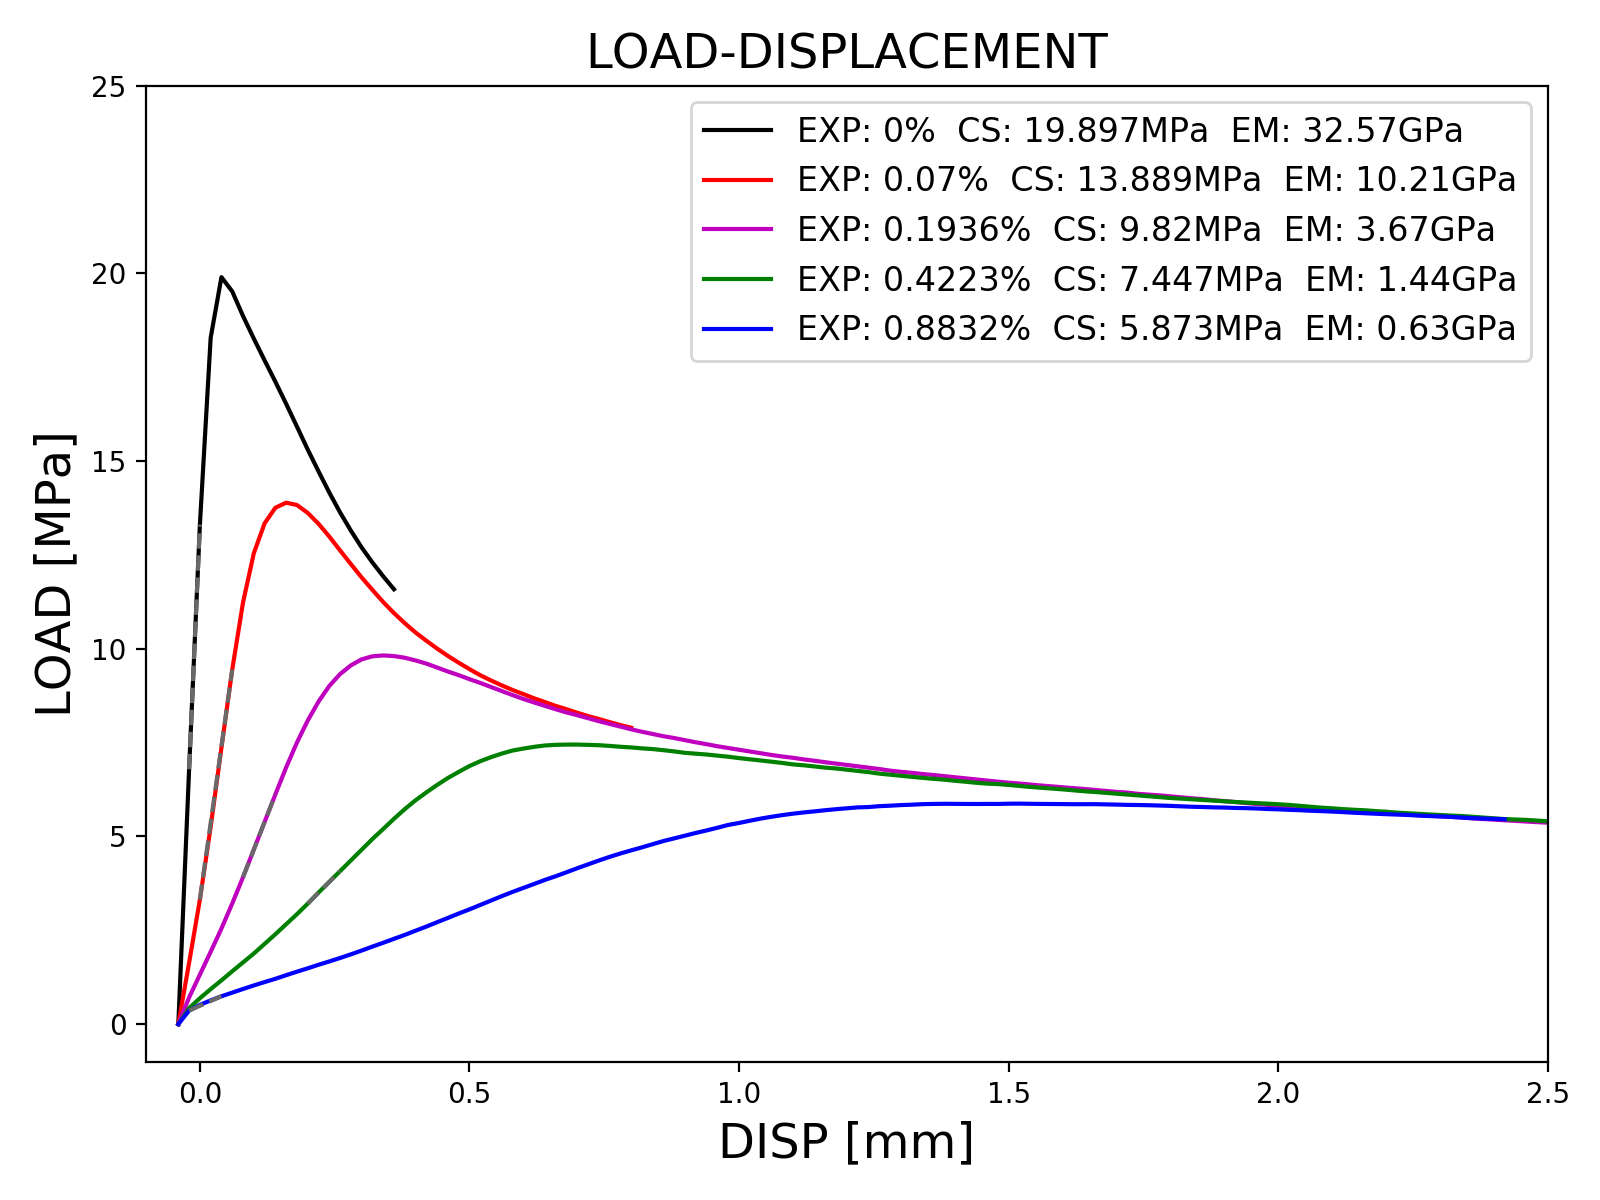
\includegraphics[width=.8\linewidth]{Files/exp_3D/ASR/S13A30P75FREE-LOAD-DISPLACEMENT.png}
  \caption{A30 P75 Free Load-Displacement}
  \label{fig:A30P75FREE_LD}
\end{figure}

Shown in Figure \ref{AncaLoadDisp} are comparisons between the stress-strain relationships of four cylinder concrete specimens experimentally tested by Giaccio et al\cite{Giaccio}, in fixed boudary condition. Those numerically using three alternative concrete compression stress-strain response models—namely, Hognestad parabola, Attard and Setunge model\cite{Attard}, and Popovics HSC model\cite{Thorenfeldt}.

Compare Figure \ref{AncaLoadDisp} with Figure \ref{fig:A30P75FIX_LD}, our simulation result does show a similar trend in load displacement relationship.

\begin{figure}[ht!]
\centering
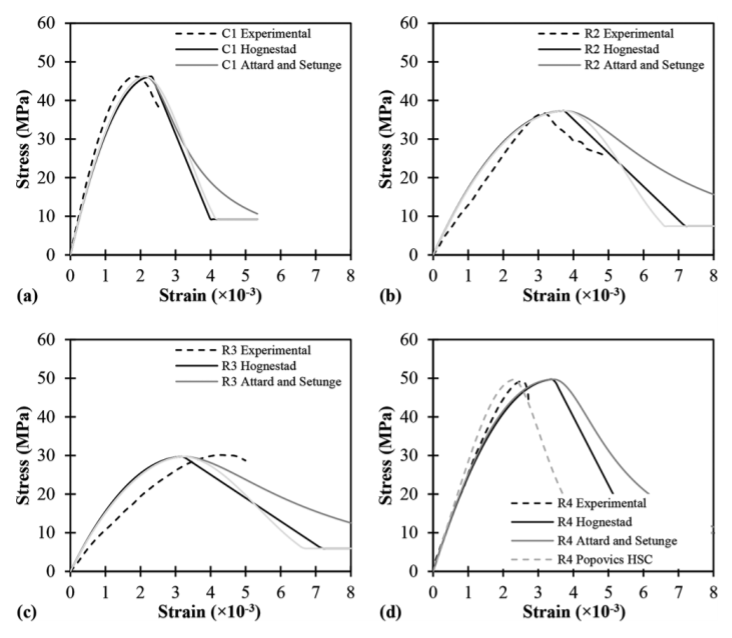
\includegraphics[width=.8\linewidth]{Reference/AncaASR.png}
  \caption{Stress-strain behavior in compression: (a) nonreactive mixture C1; (b) reactive mixture R2; (c) reactive mixture R3; and (d) reactive mixture R4. (Note: 1 kN = 0.2248 kip; 1 mm = 0.0394 in.)[Giaccio et al., 2008]}
  \label{AncaLoadDisp}
\end{figure}

Here if plot the Residual Compressive Strength obtained from fixed boundary expansion with the one dimensional gloal expansion, it can be seen that the trend is quite close with some of the experimental results, especially the results from Swamy \& Al-Asali, 1988\cite{Swamy}.

The trend of lossing in residual compressive strength along with the increasing in expanion is well presented, in Figure \ref{A30P7sss5_CS_2}. Though the model used in this simulation is not identical with the experimental one, it does show similar trend in relately ratio of residential compressive strength lossing.

\begin{figure}[ht!]
\centering
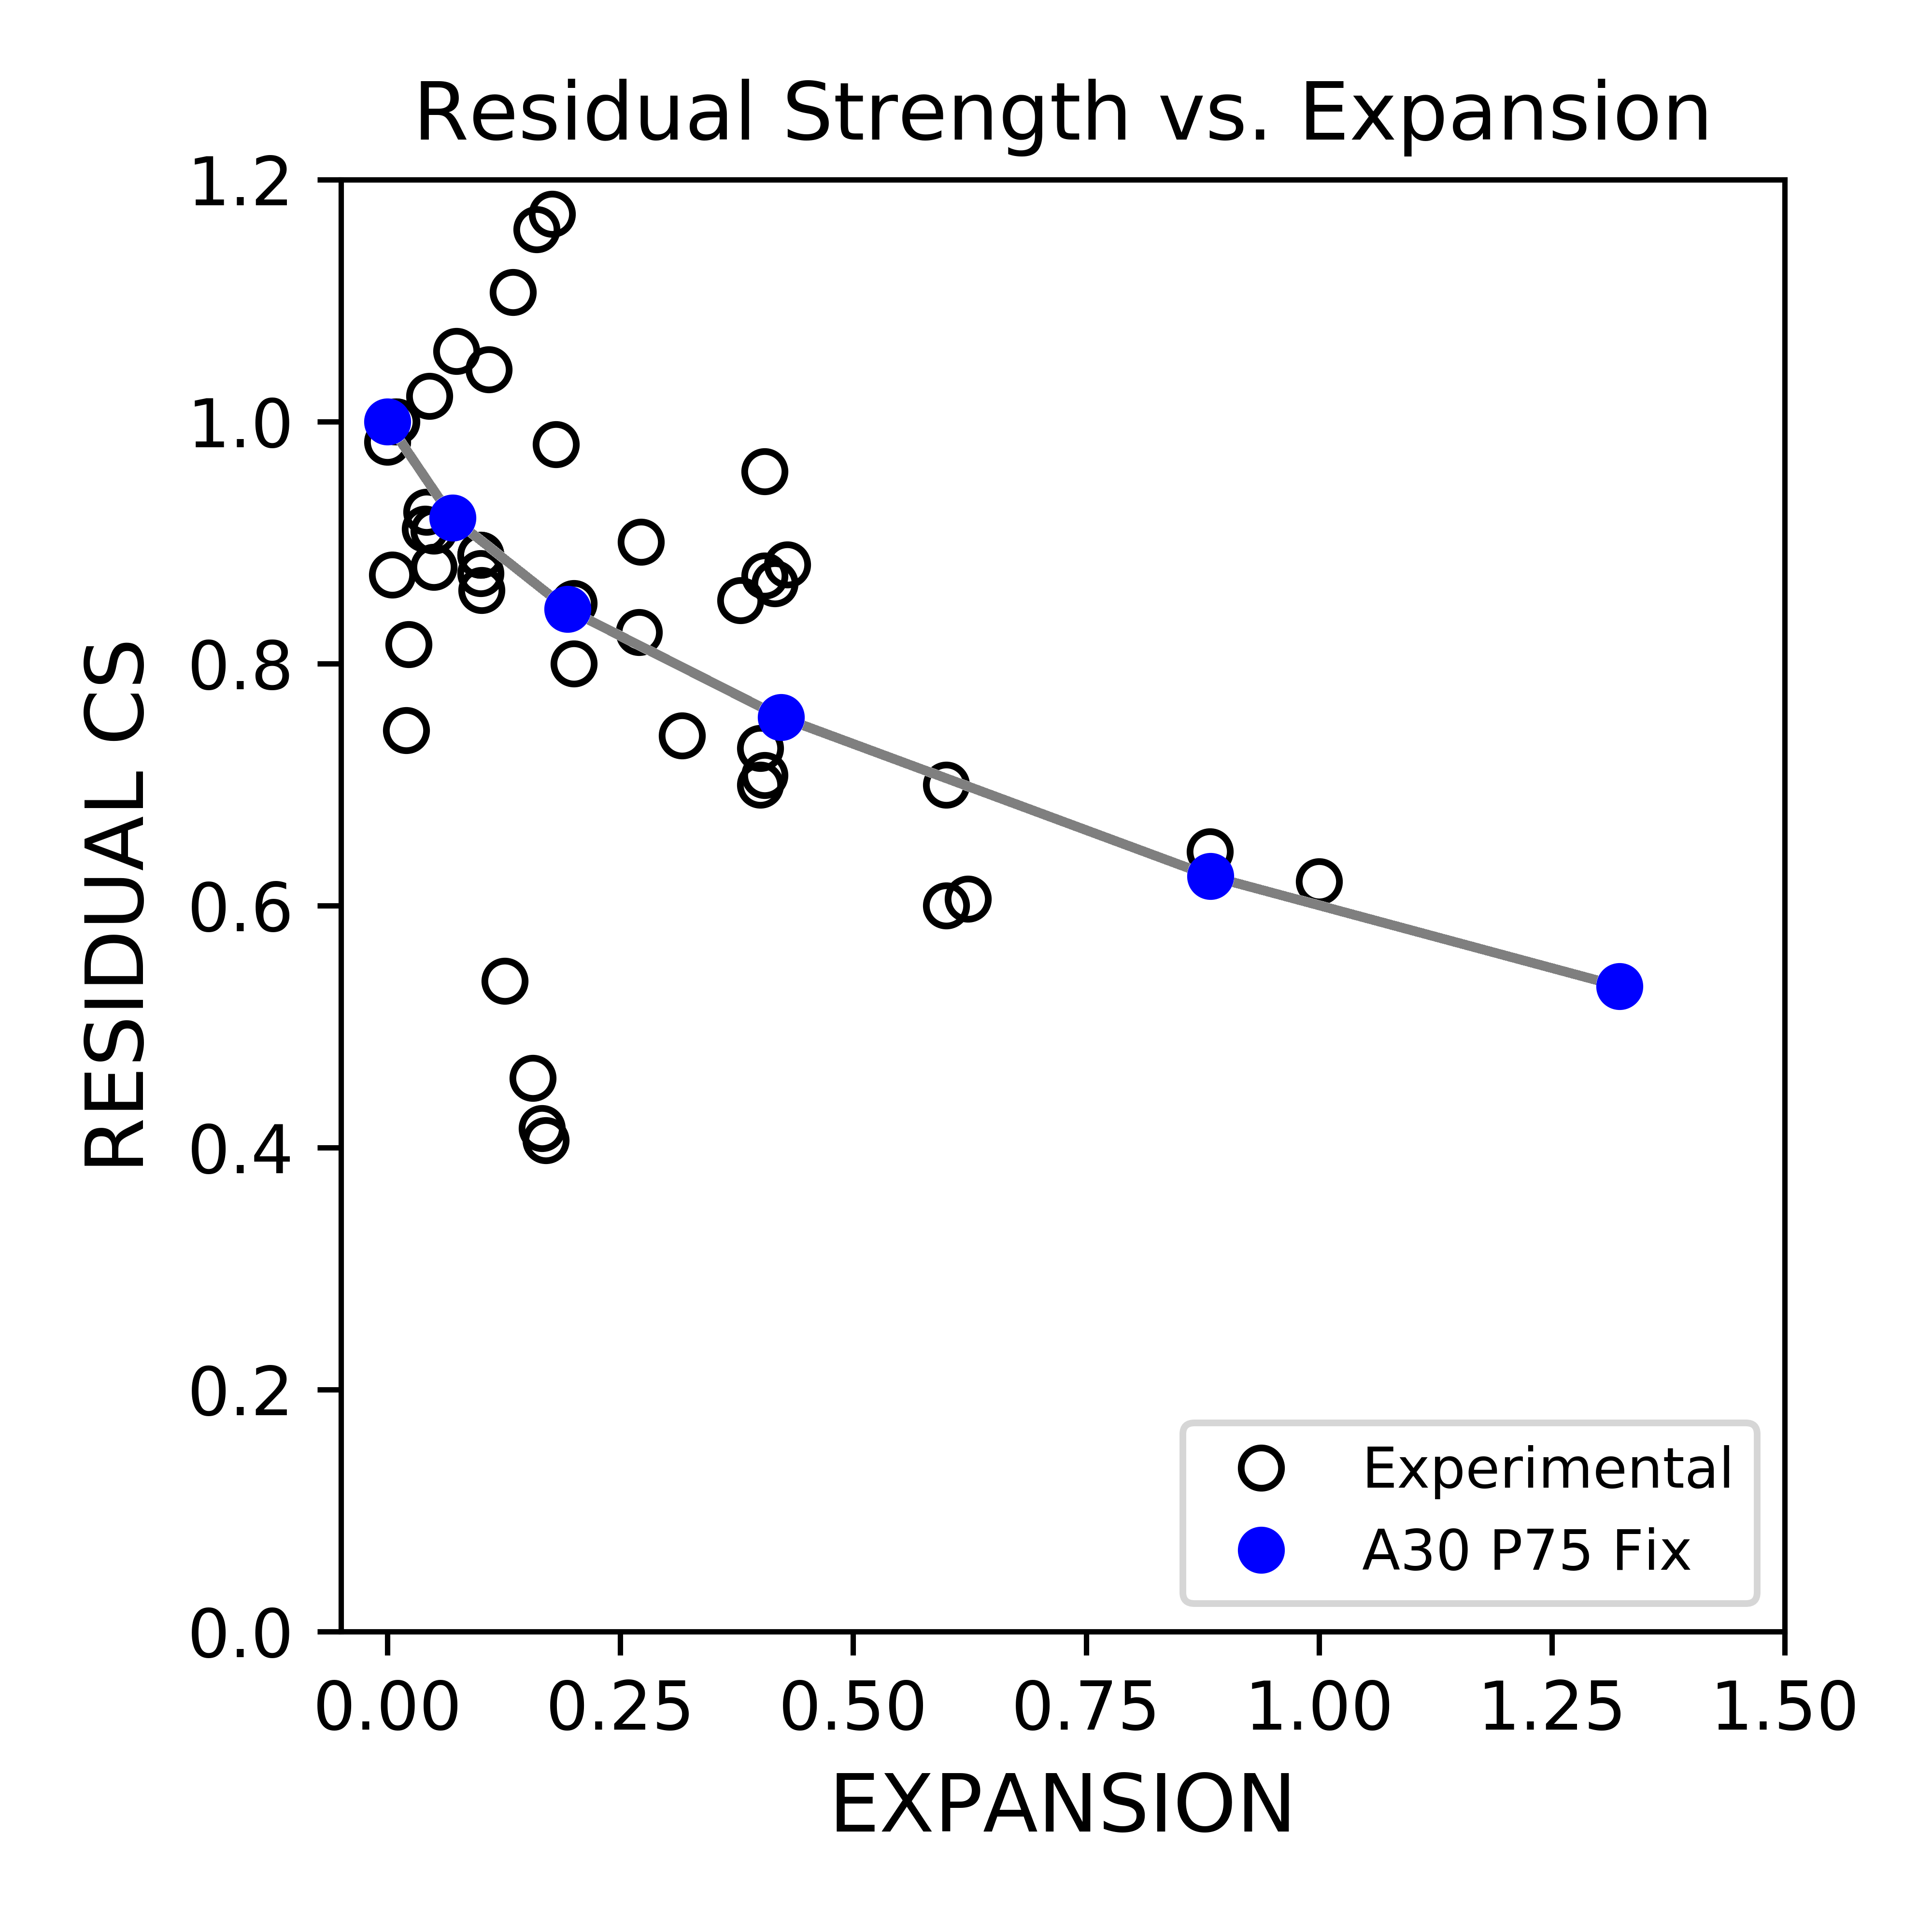
\includegraphics[width=.8\linewidth]{Files/CS_plot/ASRCS1.png}
  \caption{A30 P75 Compressive Strength Comparing With Experimental Results}
  \label{A30P7sss5_CS_2}
\end{figure}



However, if plot the residual elastic modulus along with the increasing in expanion, shown in Figure \ref{A30P75_EM_2}, the losses in our simulation is significantly higher than experimental result. Start from very low expansion amout the simulated residual elastic modulus dropped to over 80\% losses.

One of the assumption is that in our simulation model, once crack is opened, it would be set as void with no abilitu to carry any force before closing the gap totally. However, this may not be true in really, for ASR, gel is generated and filling in part of the cracks, especially cracks between aggregate and surrounding paste. The mechanical properties of ASR gel is still under discussion, and for certainly they should be considered when simulating the mechanical properties of ASR damaged models. Simulation and for expansion and loading in ASR still requires to be improved to represent the mechanical properties losses more percisely in reality.


\begin{figure}[ht!]
\centering
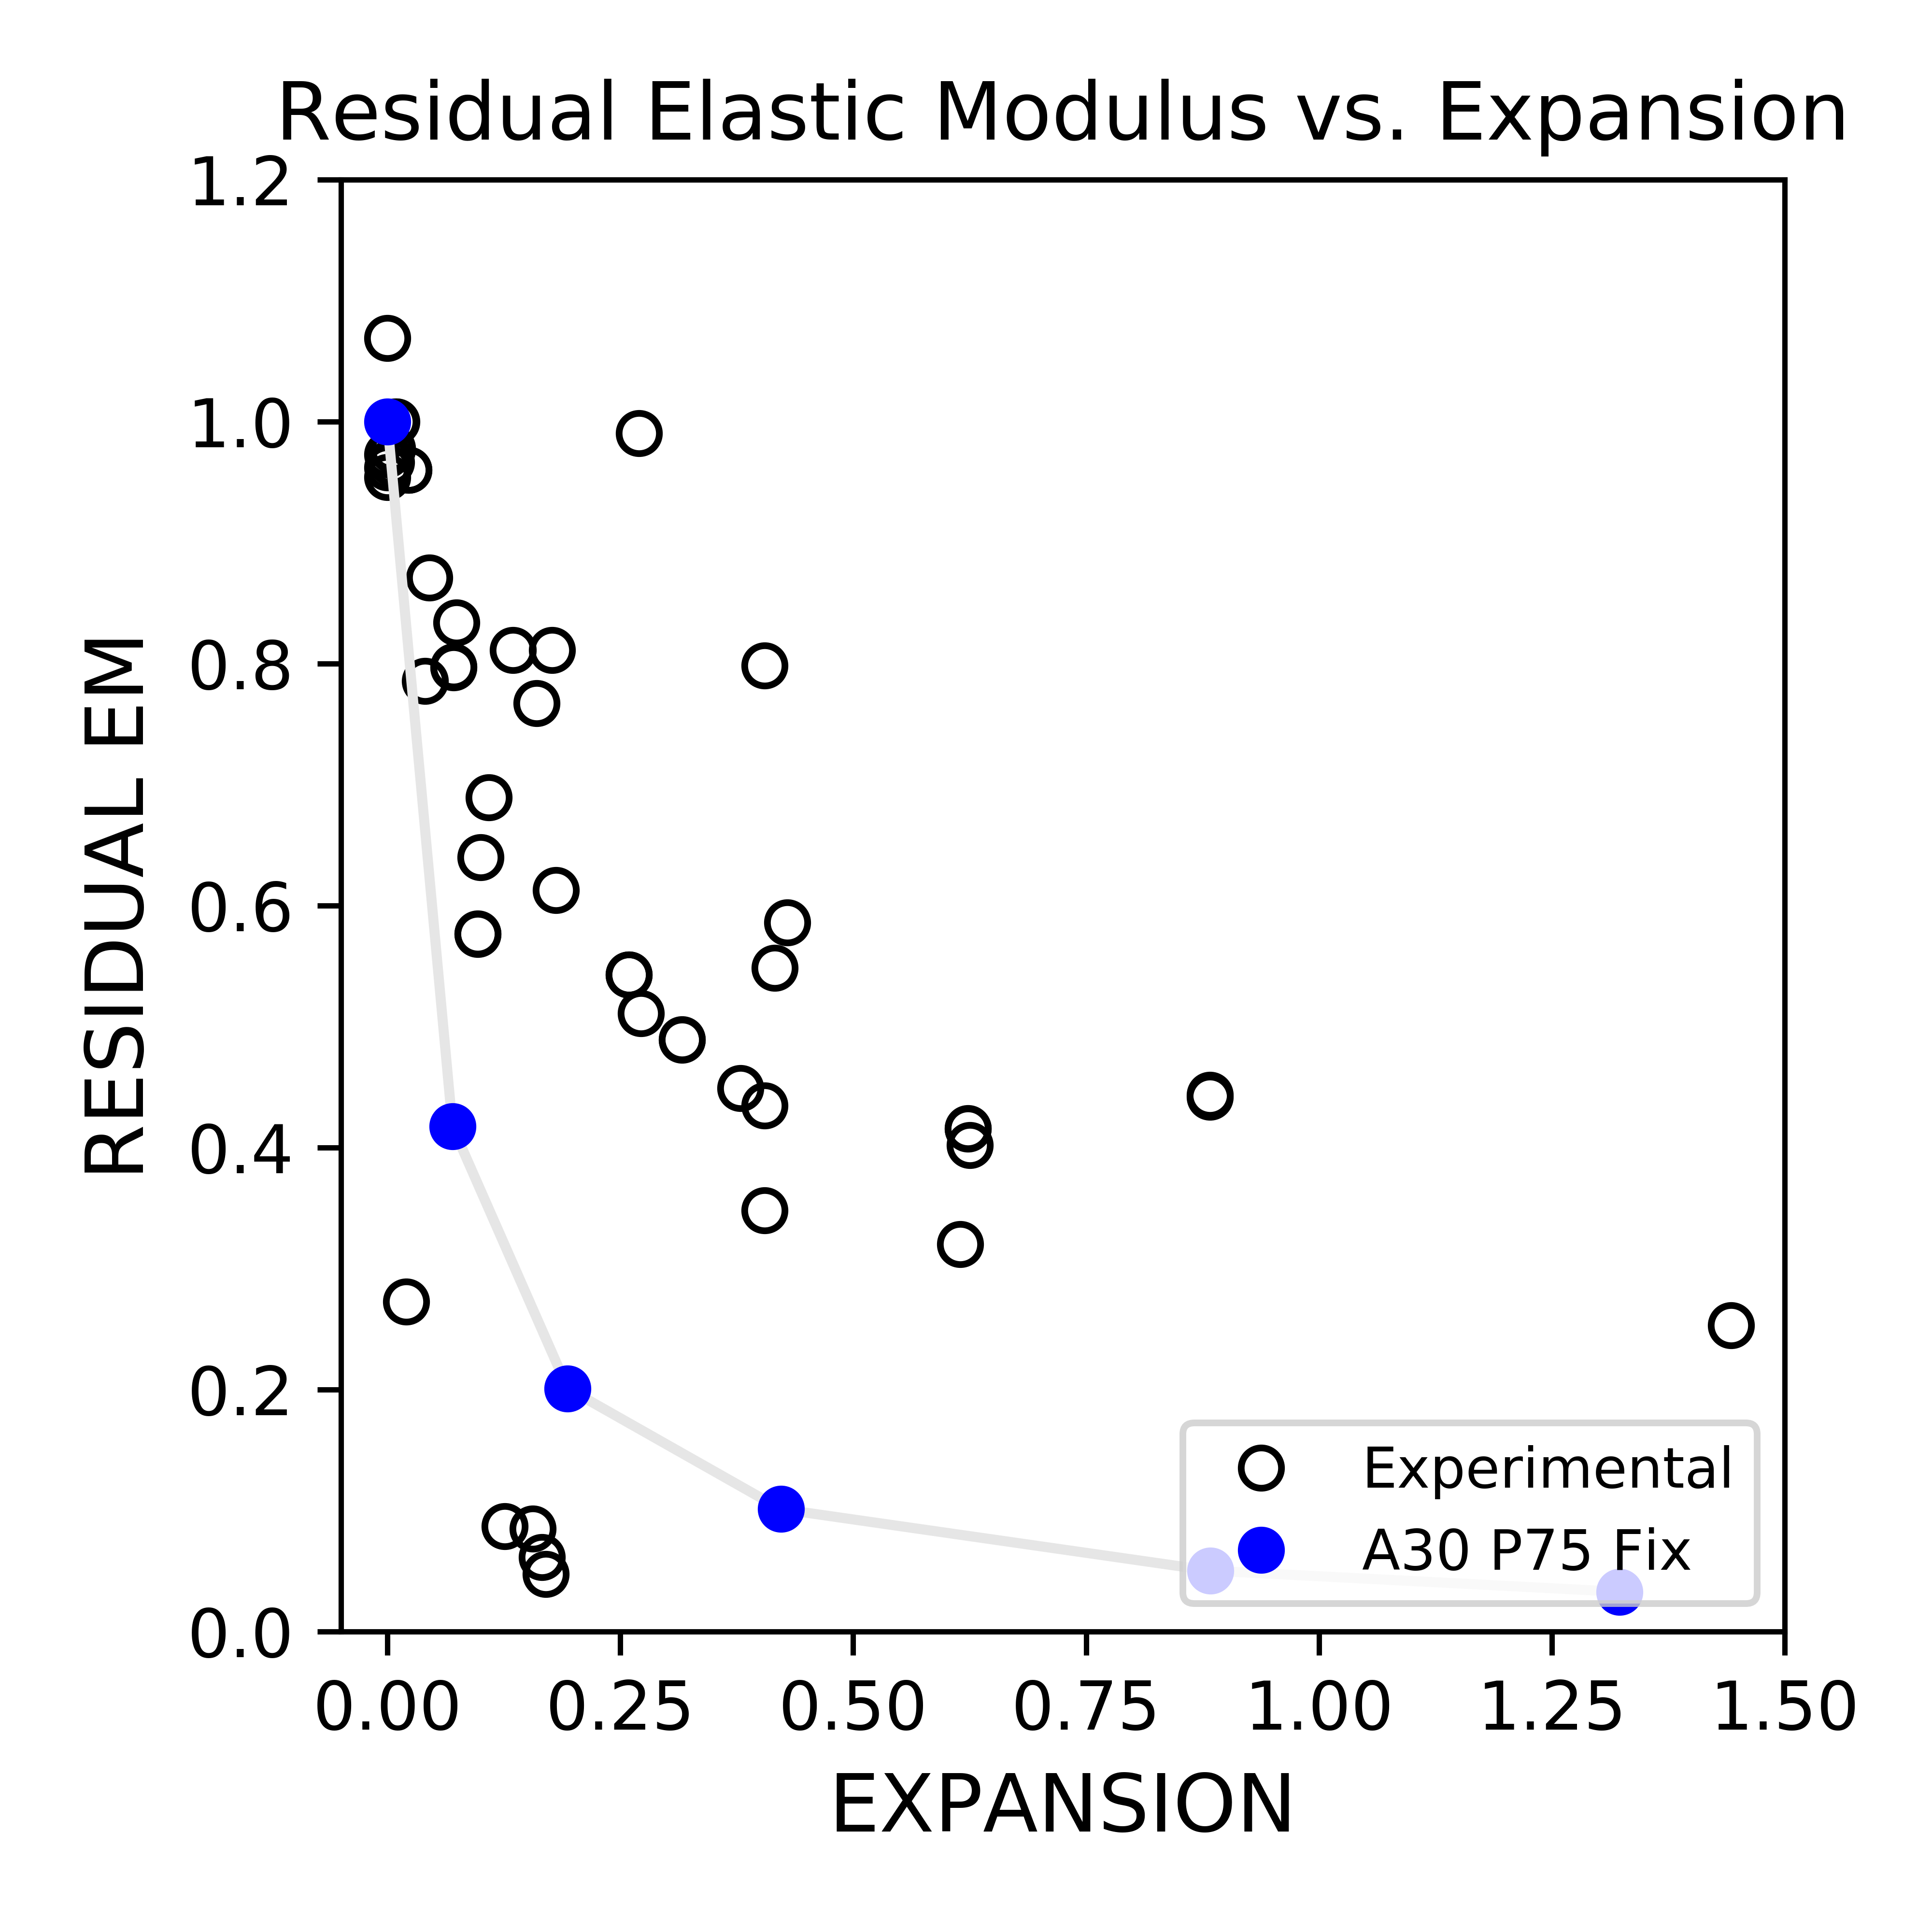
\includegraphics[width=.8\linewidth]{Files/CS_plot/ASREM1.png}
  \caption{A30 P75 Elastic Modulus Comparing With Experimental Results}
  \label{A30P75_EM_2}
\end{figure}

% \begin{table}[ht!]
% \centering
% \begin{tabular}{ ||p{2cm}|p{2cm}|p{2cm}|p{3cm}|p{3cm}|| }
%  \hline
%   Initial Strain (Each Step) & Expanding Steps & Final Expansion [\%] & Maximum Compressive Strength in Fix Loading Condition [MPa] & Maximum Compressive Strength in Free Loading Condition [MPa]\\ [0.5ex]
%  \hline\hline
%   0 & 0 & 0 & 29.987 & 19.897\\
%   0.0002 & 20 & 0.0699 & 27.601 & 13.889\\
%   0.0005 & 20 & 0.1936 & 25.339 & 9.8203\\
%   0.001 & 20 & 0.4223 & 22.667 & 7.4466\\
%   0.002 & 20 & 0.8832 & 18.725 & 5.8732 \\
%   0.003 & 20 & 1.3224 & 15.993 &\\
%
%  \hline
% \end{tabular}
% \caption{One Dimensional Expansion Ratio in Single ASR Model Simulation}
% \label{table:ASR_30_EXP}
% \end{table}



\clearpage

Other uni-axial loading simulation results for expanded models in different cases are also summarized below.

For ASR expanded model with 30\% coarse aggregate (of which 25\% are ASR reactive), shown in Figure \ref{fig:A30P25_model}, the Load-Displacement curve is shown in Figure \ref{fig:A30P25FIX_LD}.

%A30P25FIX
\begin{figure}[ht]
\centering
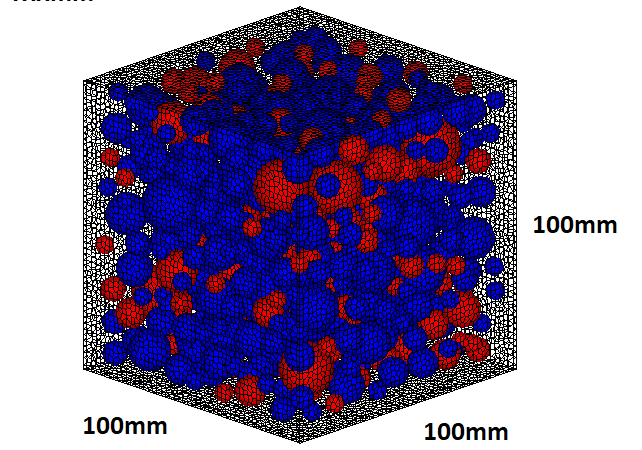
\includegraphics[width=.3\linewidth]{Files/Aggregate/A30P25.png}
  \caption{30\% Coarse Aggregate}
  \label{fig:A30P25_model}
\end{figure}

\begin{figure}[ht]
\centering
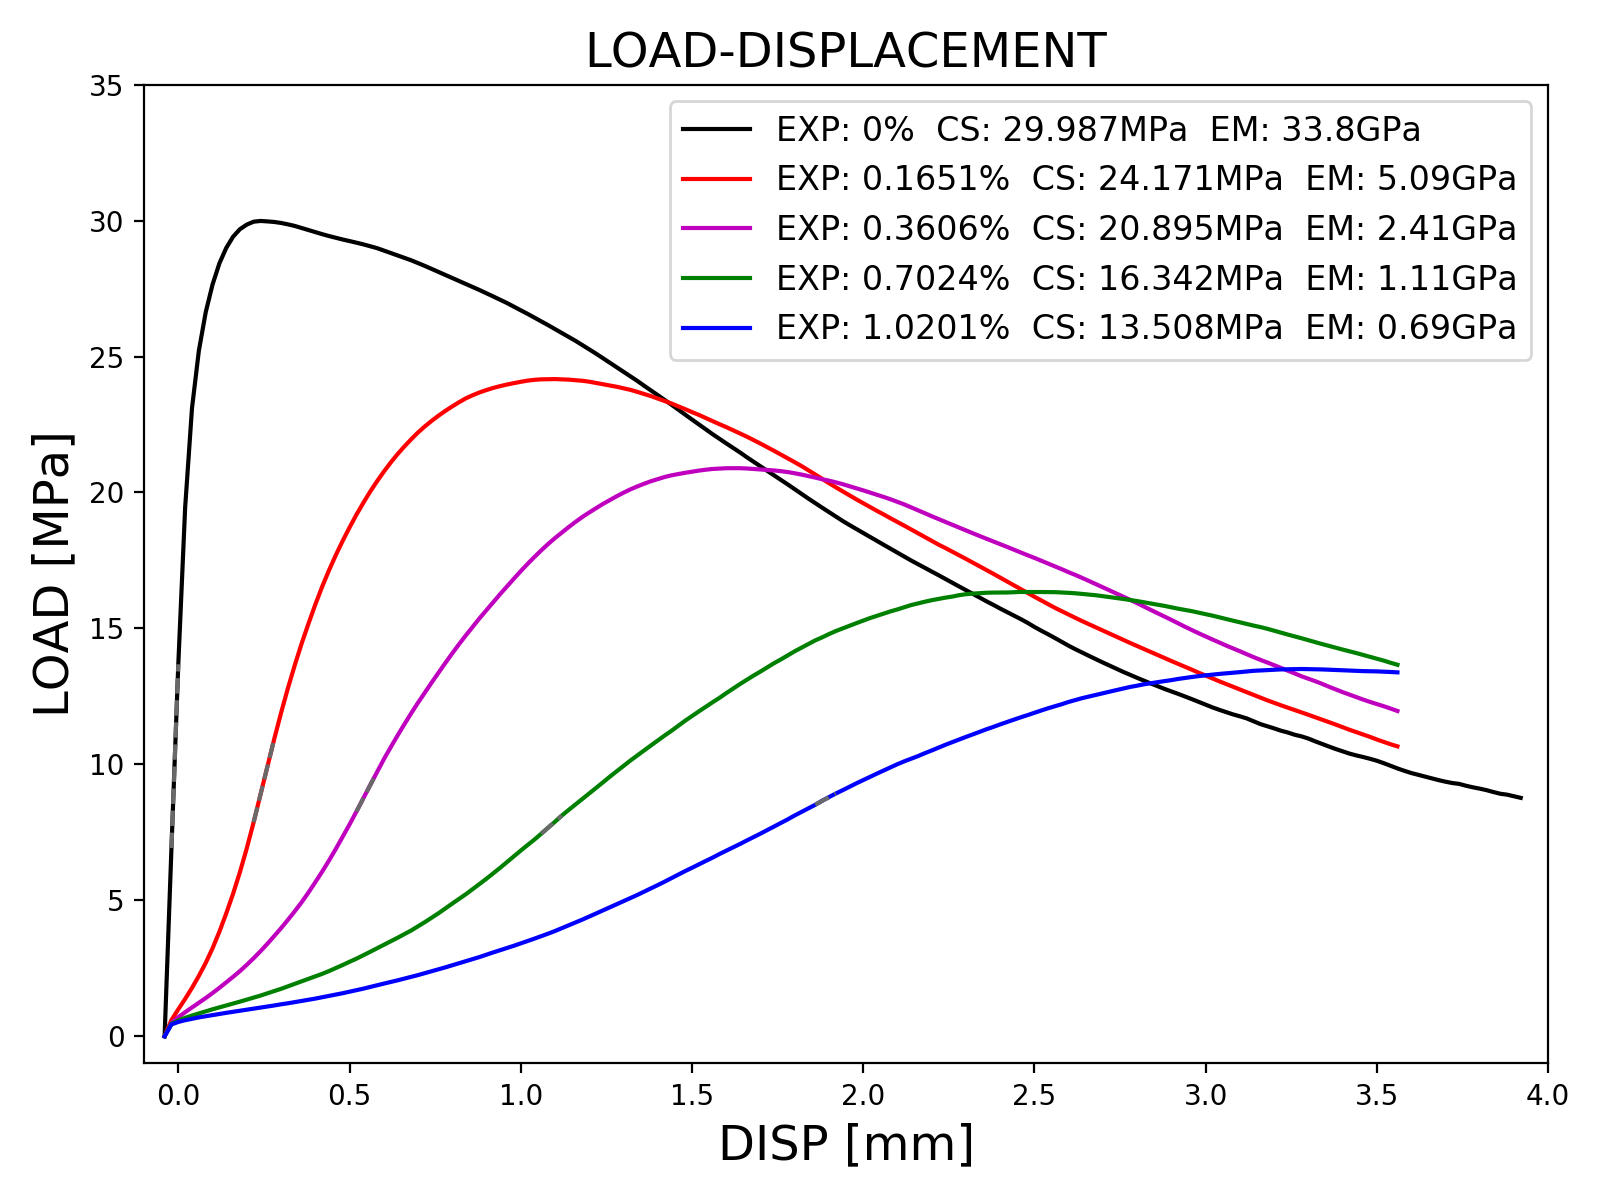
\includegraphics[width=.8\linewidth]{Files/exp_3D/ASR/S13A30P25FIX-LOAD-DISPLACEMENT.png}
  \caption{A30 P25 Fix Load-Displacement}
  \label{fig:A30P25FIX_LD}
\end{figure}

\clearpage

For ASR expanded model with 15\% coarse aggregate (of which 75\% are ASR reactive), shown in Figure \ref{fig:A15P75_model}, the Load-Displacement curve is shown in Figure \ref{fig:A15P75FIX_LD}.

%A15P75FIX

\begin{figure}[ht]
\centering
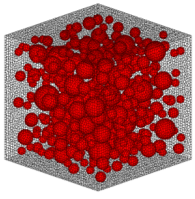
\includegraphics[width=.3\linewidth]{Files/Aggregate/A15.png}
  \caption{15\% Coarse Aggregate}
  \label{fig:A15P75_model}
\end{figure}

\begin{figure}[ht]
\centering
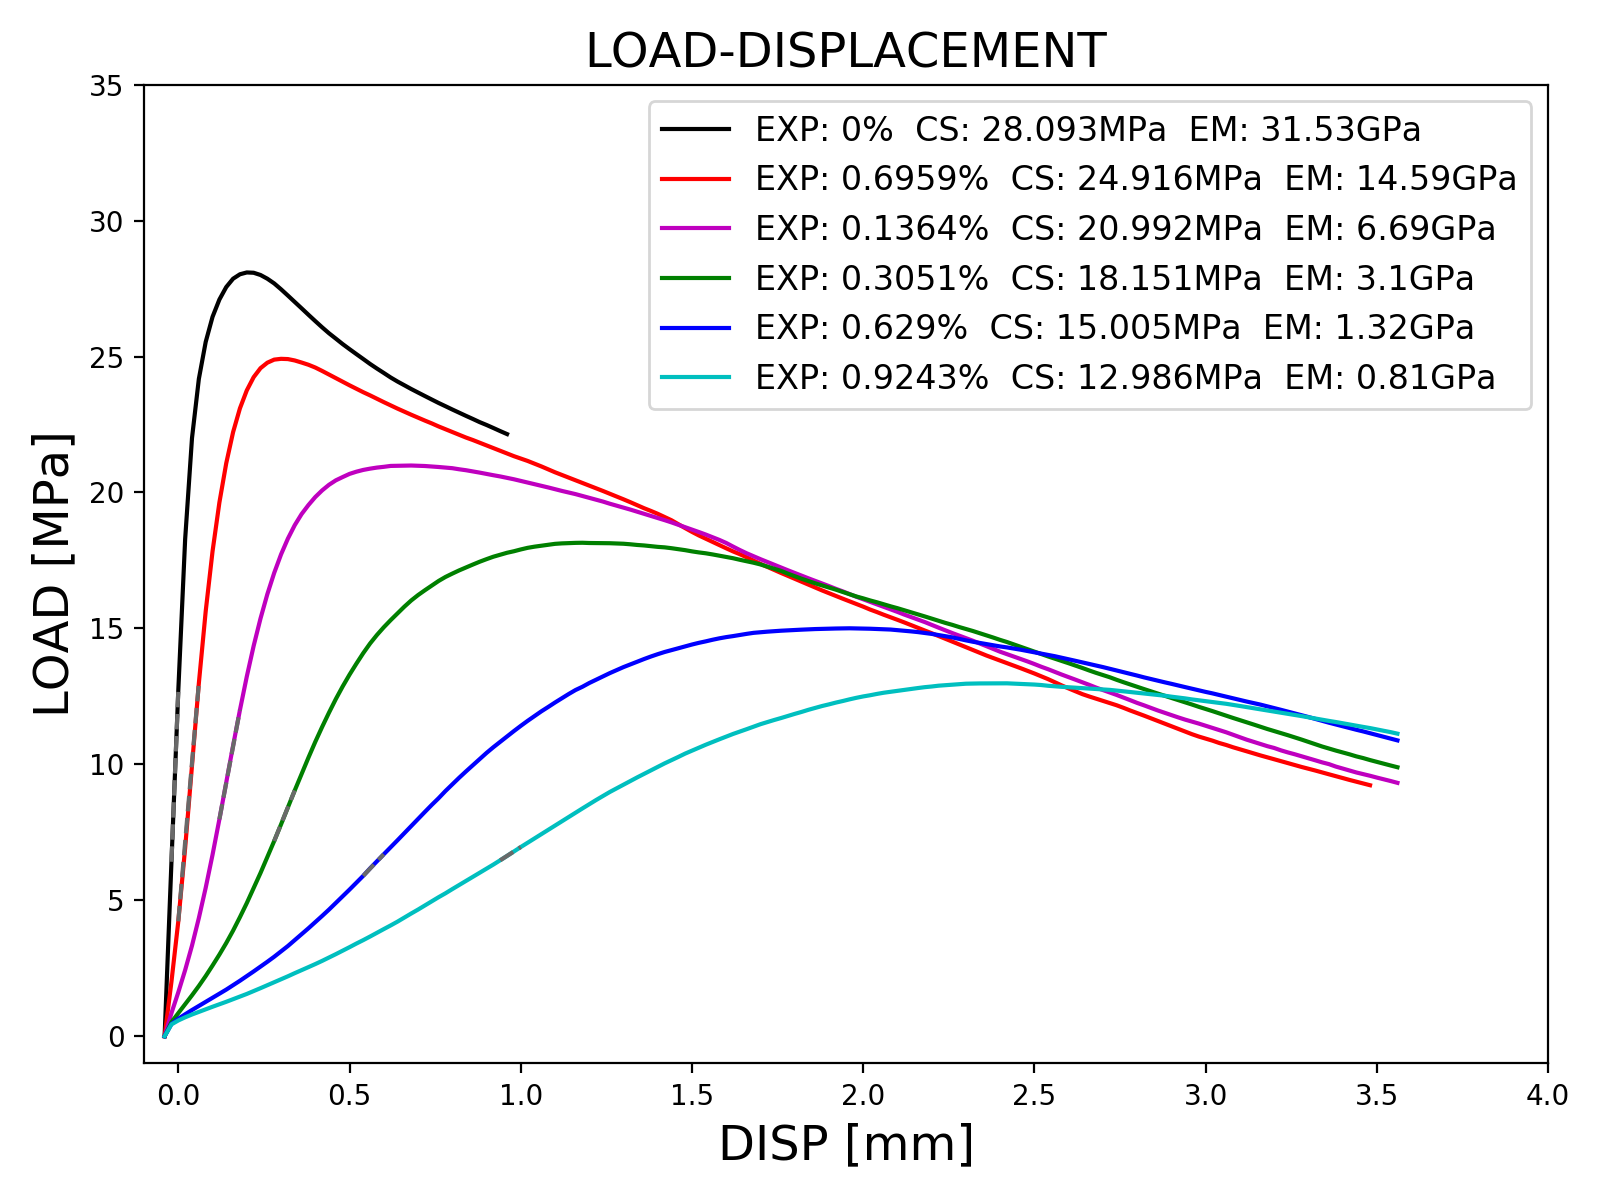
\includegraphics[width=.8\linewidth]{Files/exp_3D/ASR/S13A15P75FIX-LOAD-DISPLACEMENT.png}
  \caption{A15 P75 Fix Load-Displacement}
  \label{fig:A15P75FIX_LD}
\end{figure}

\clearpage

The simulation result in residual compressive strength here is plotted, as in Figure \ref{ASR_CS_summary}, which can be seen that in ASR simulation, the decresaing trend in compressive strength is influenced by factores such as percentage of coarse aggregate, and percentage of reactive aggregate.

\begin{figure}[ht!]
\centering
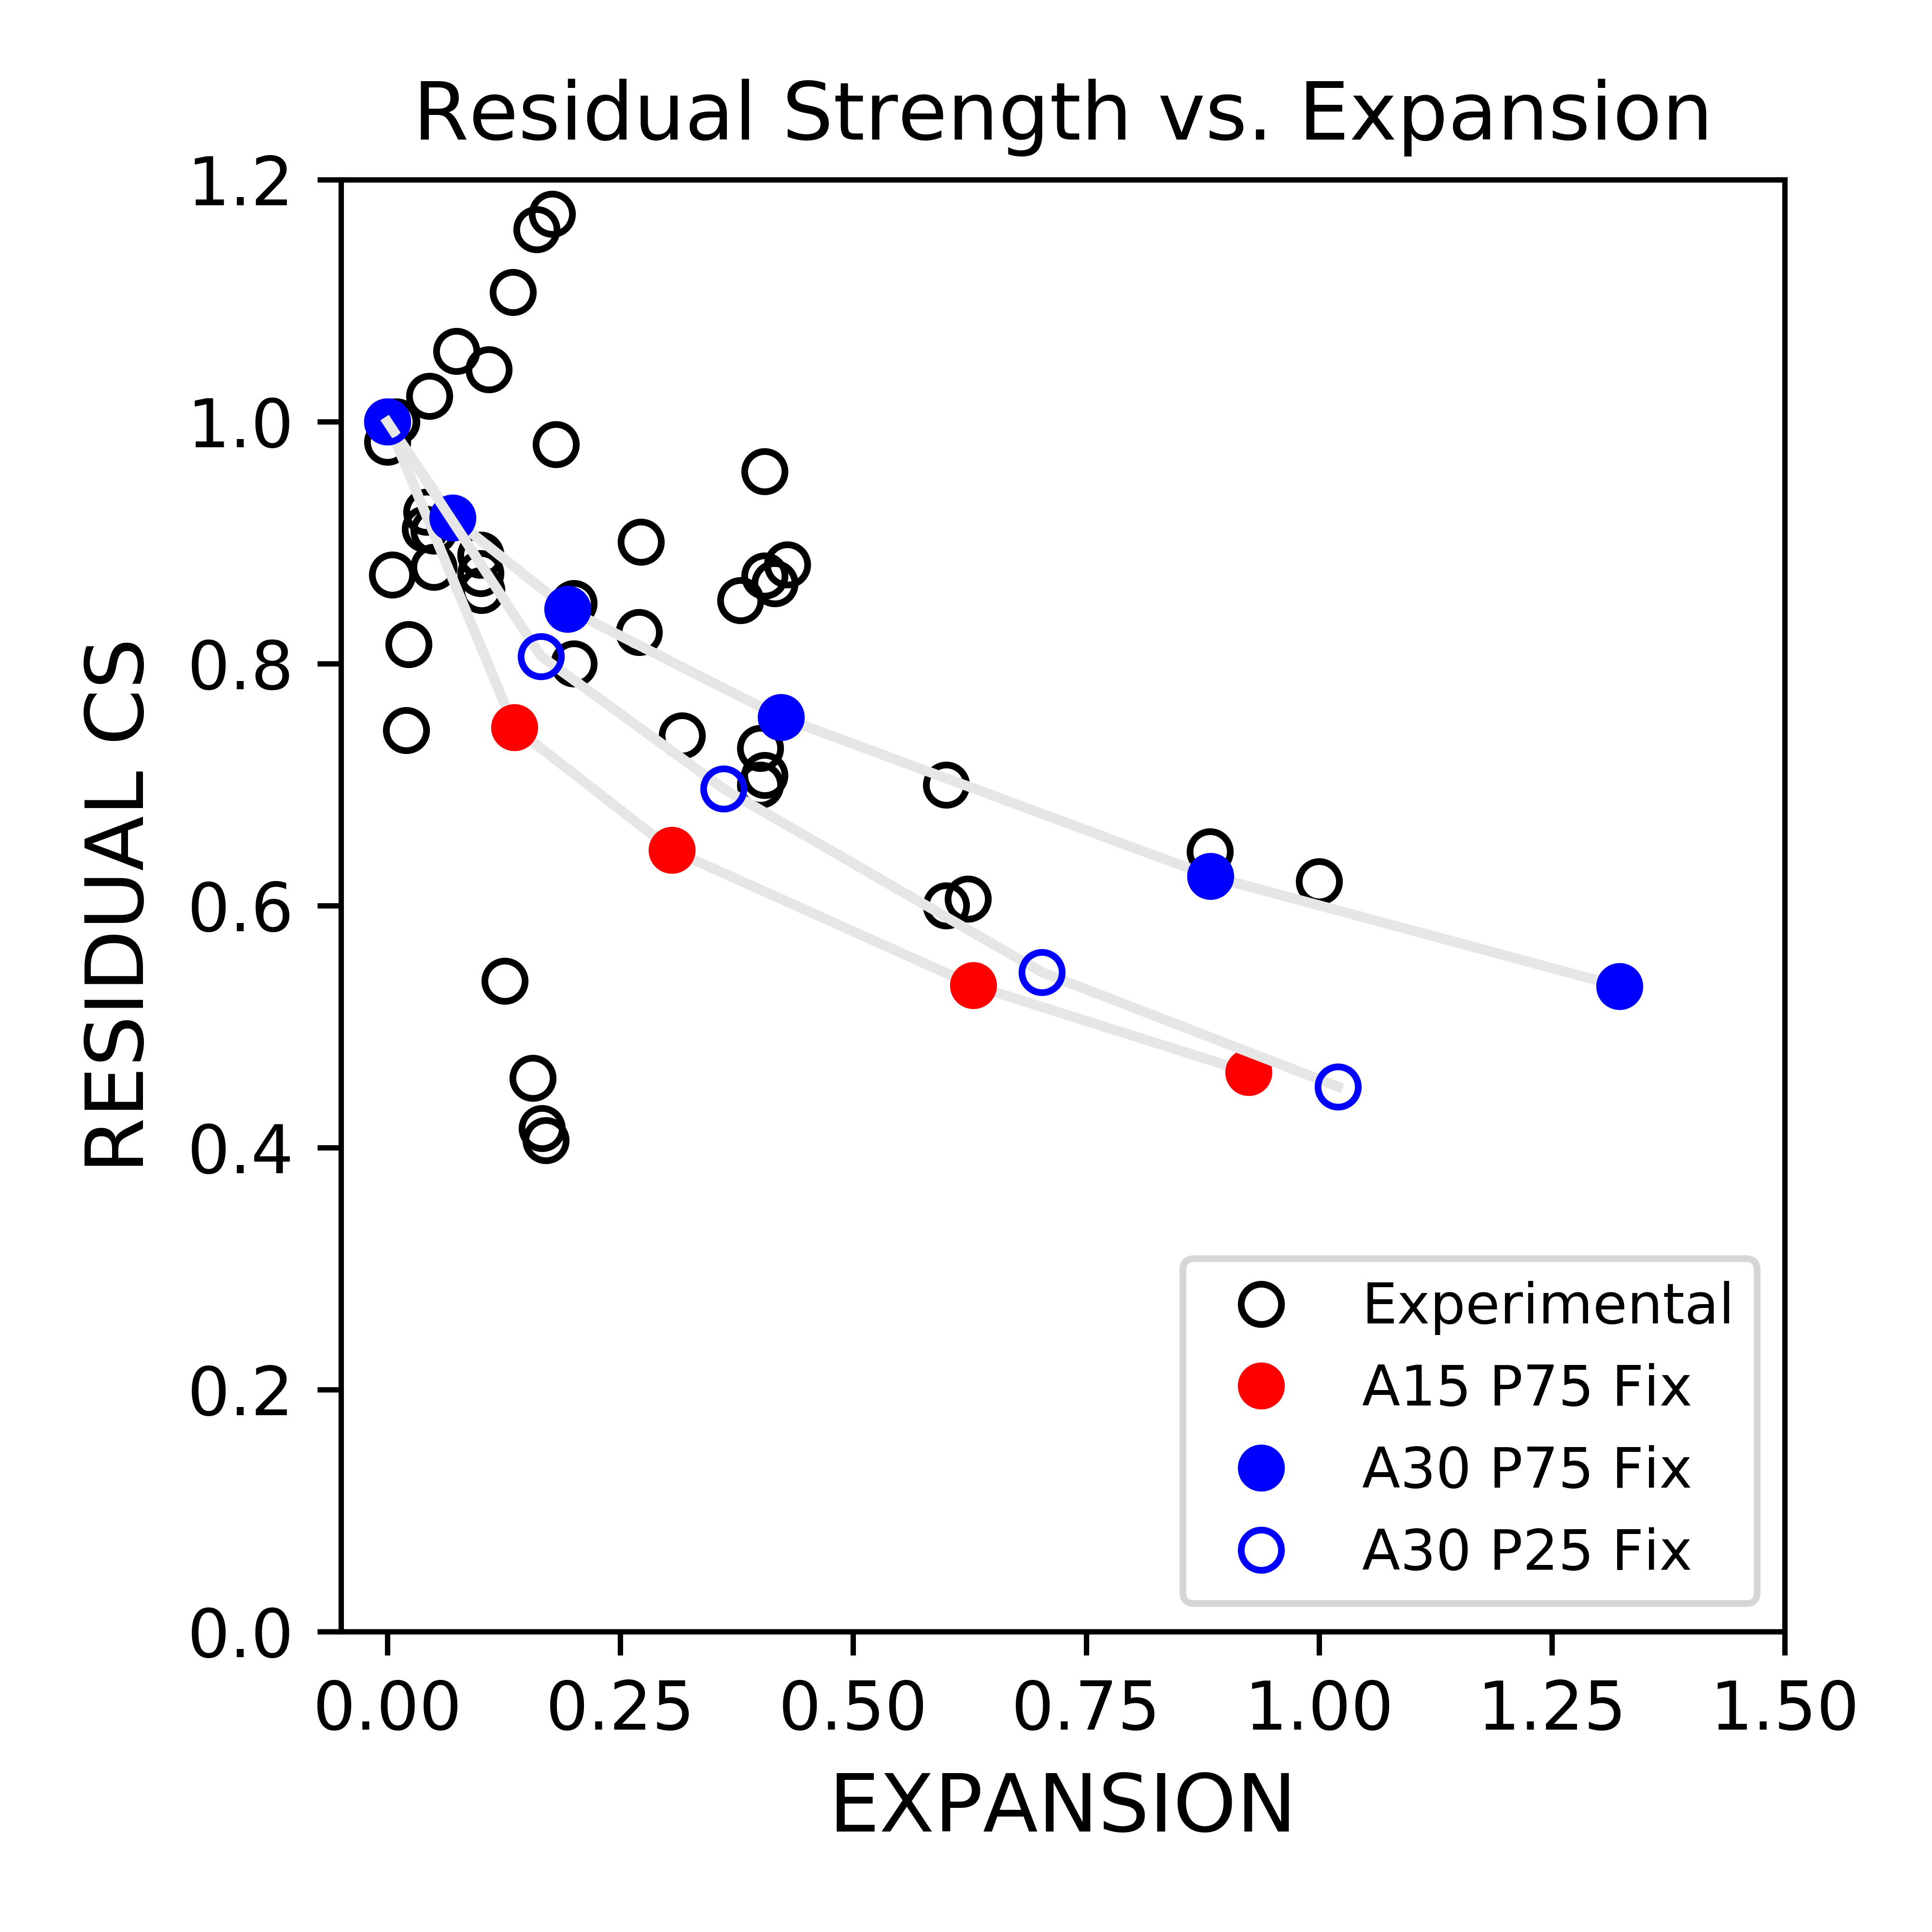
\includegraphics[width=.8\linewidth]{Files/CS_plot/ASRCS_all.png}
  \caption{ASR Compressive Strength Comparing With Experimental Results}
  \label{ASR_CS_summary}
\end{figure}

\begin{figure}[ht!]
\centering
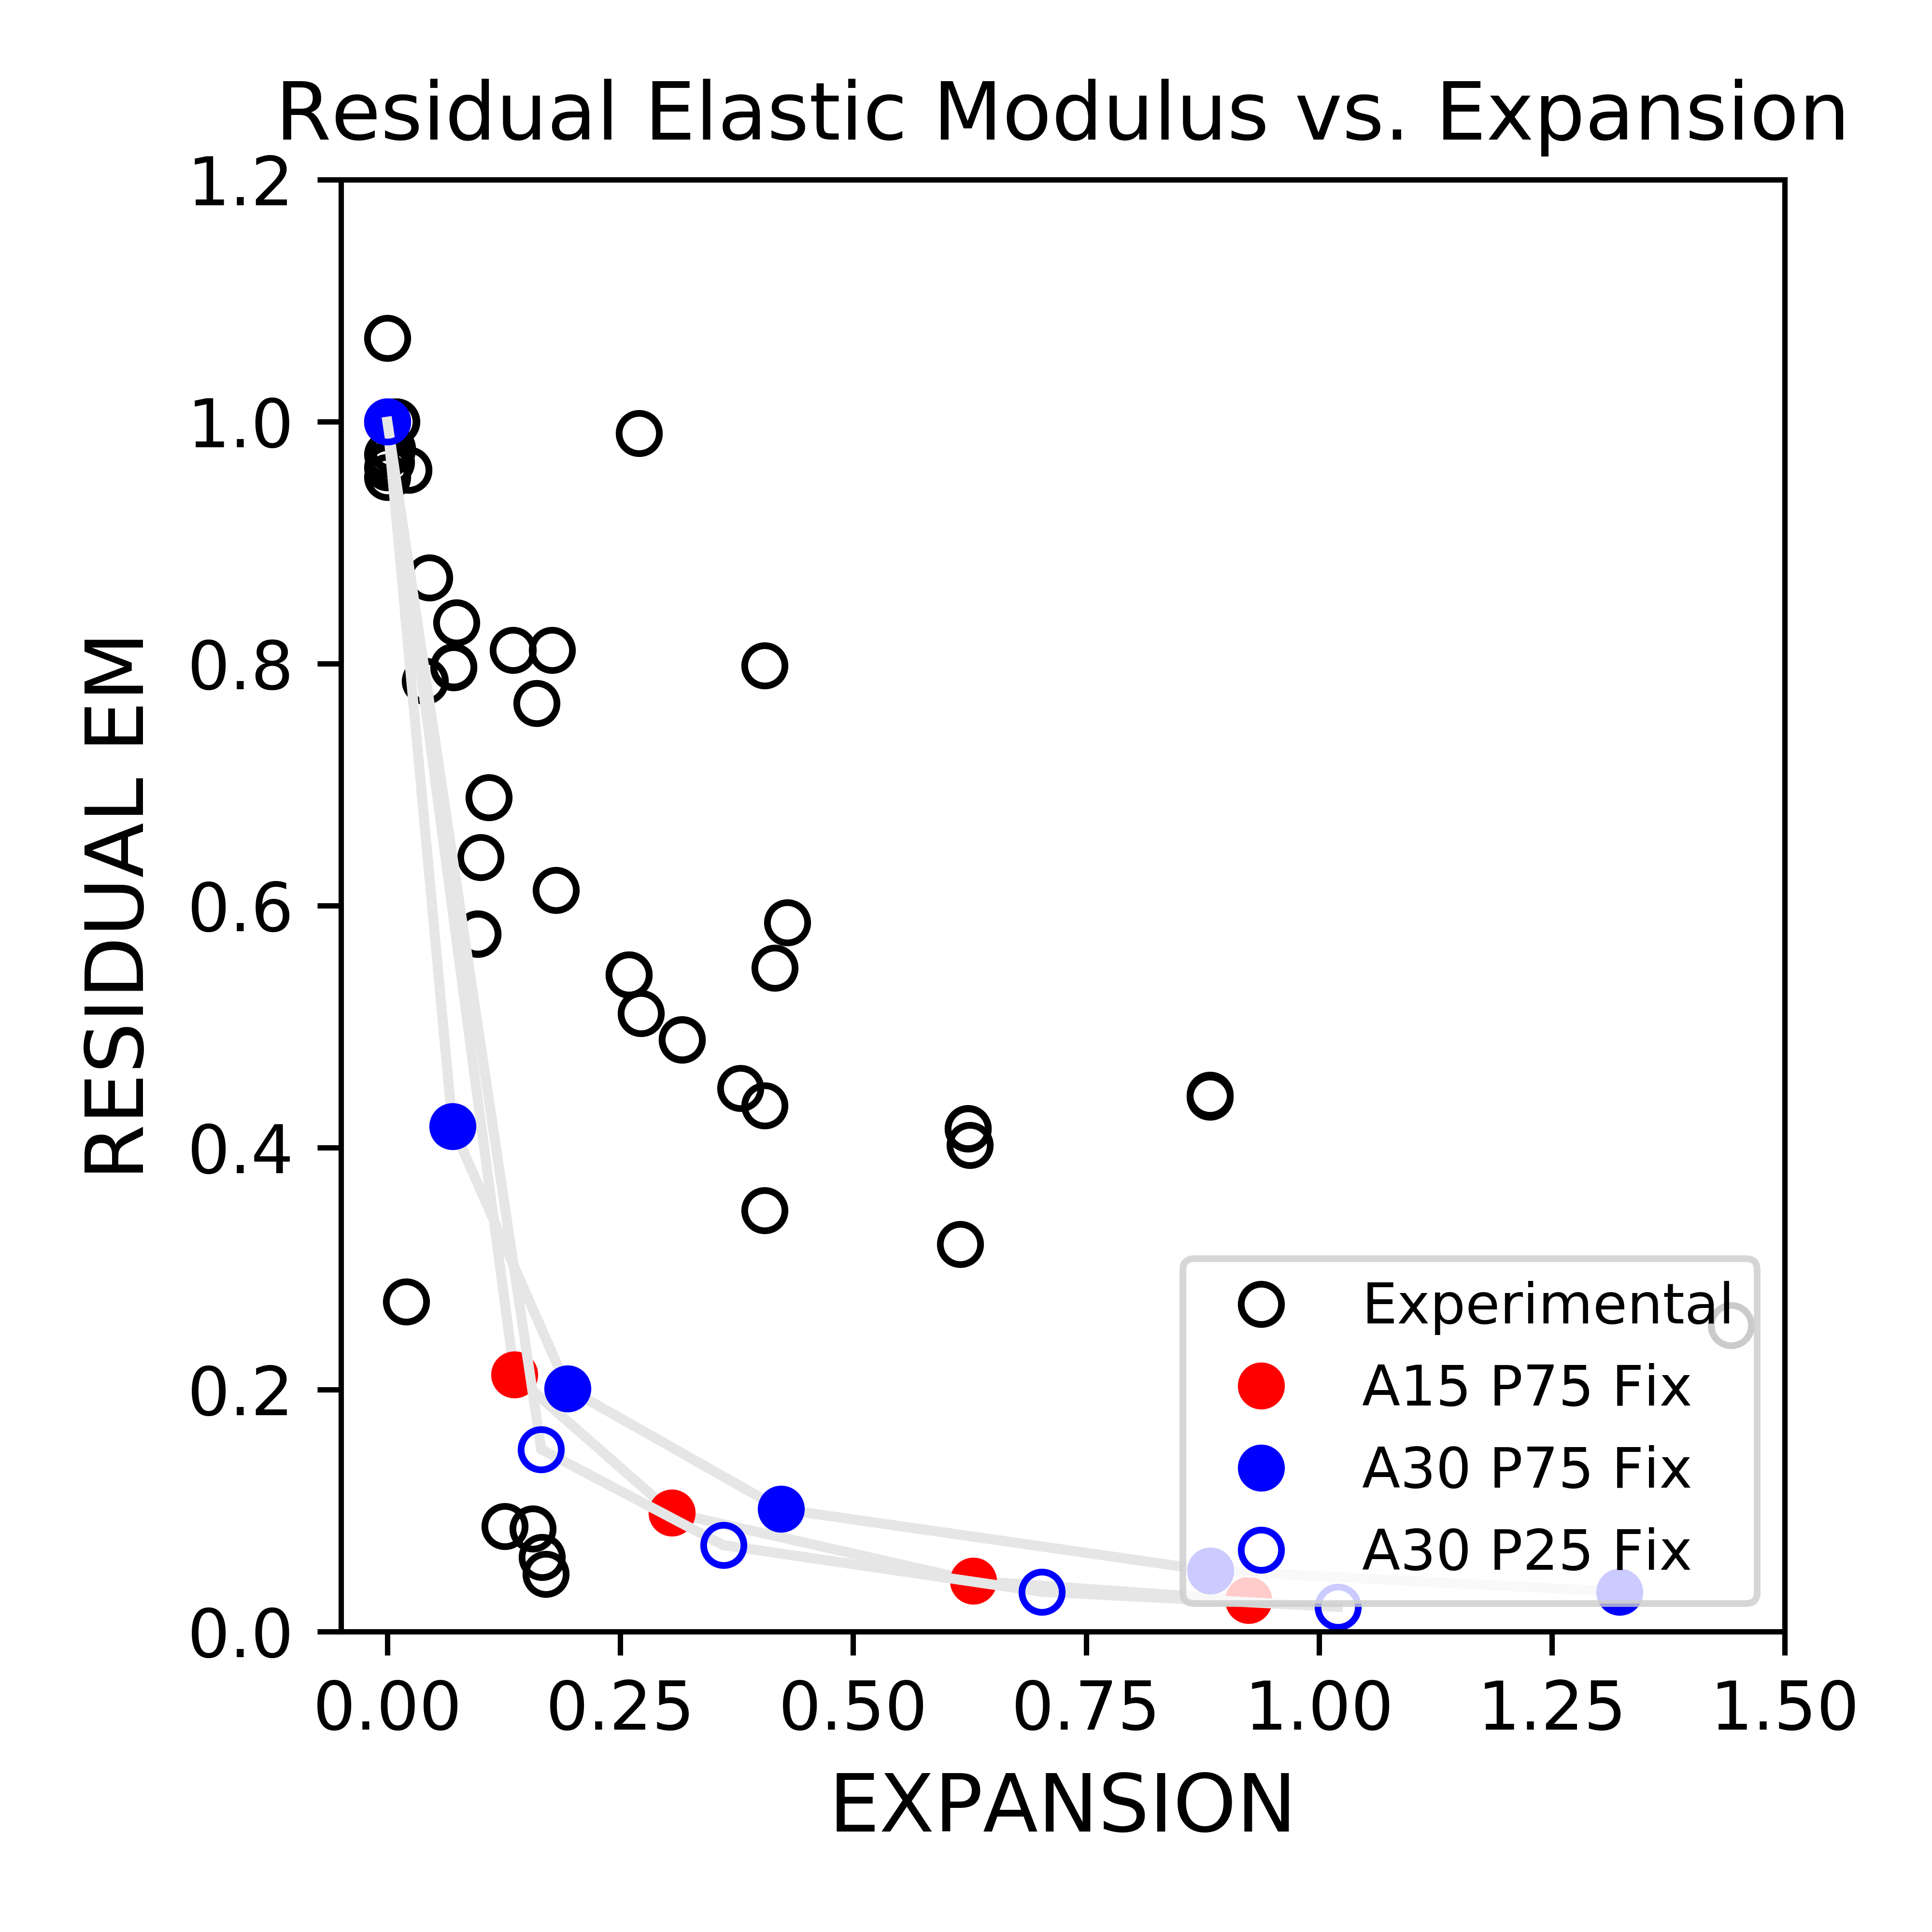
\includegraphics[width=.8\linewidth]{Files/CS_plot/ASREM_all.png}
  \caption{ASR Elastic Modulus Comparing With Experimental Results}
  \label{ASR_EM_summary}
\end{figure}

When looking at fix boundary loading, the simulation result shown in Figure \ref{ASR_CS_summary} is relatively close to some of the experimental results, as all experimental results here were loaded with fixed boundary condition.

In Figure \ref{ASR_EM_summary} it can be seen that the early losses in elastic modulus is sighnificantly higher than experimental result for all cases, which indicate that further adjustment may required in material properties of expansion damaged concrete model.

As shown in Figure \ref{ASRA30vsA15_cs}, if comparing 30\% coarse aggregate results(of which 75\% are ASR reactive), which are labeled as A30 P75, and 15\% coarse aggregate results(of which 75\% are ASR reactive), which are labeled as A15 P75, it can be seen that the residual compressive strength in 15\% coarse aggregate cases are relative lower than the 30\% coarse aggregate cases.

\begin{figure}[ht!]
\centering
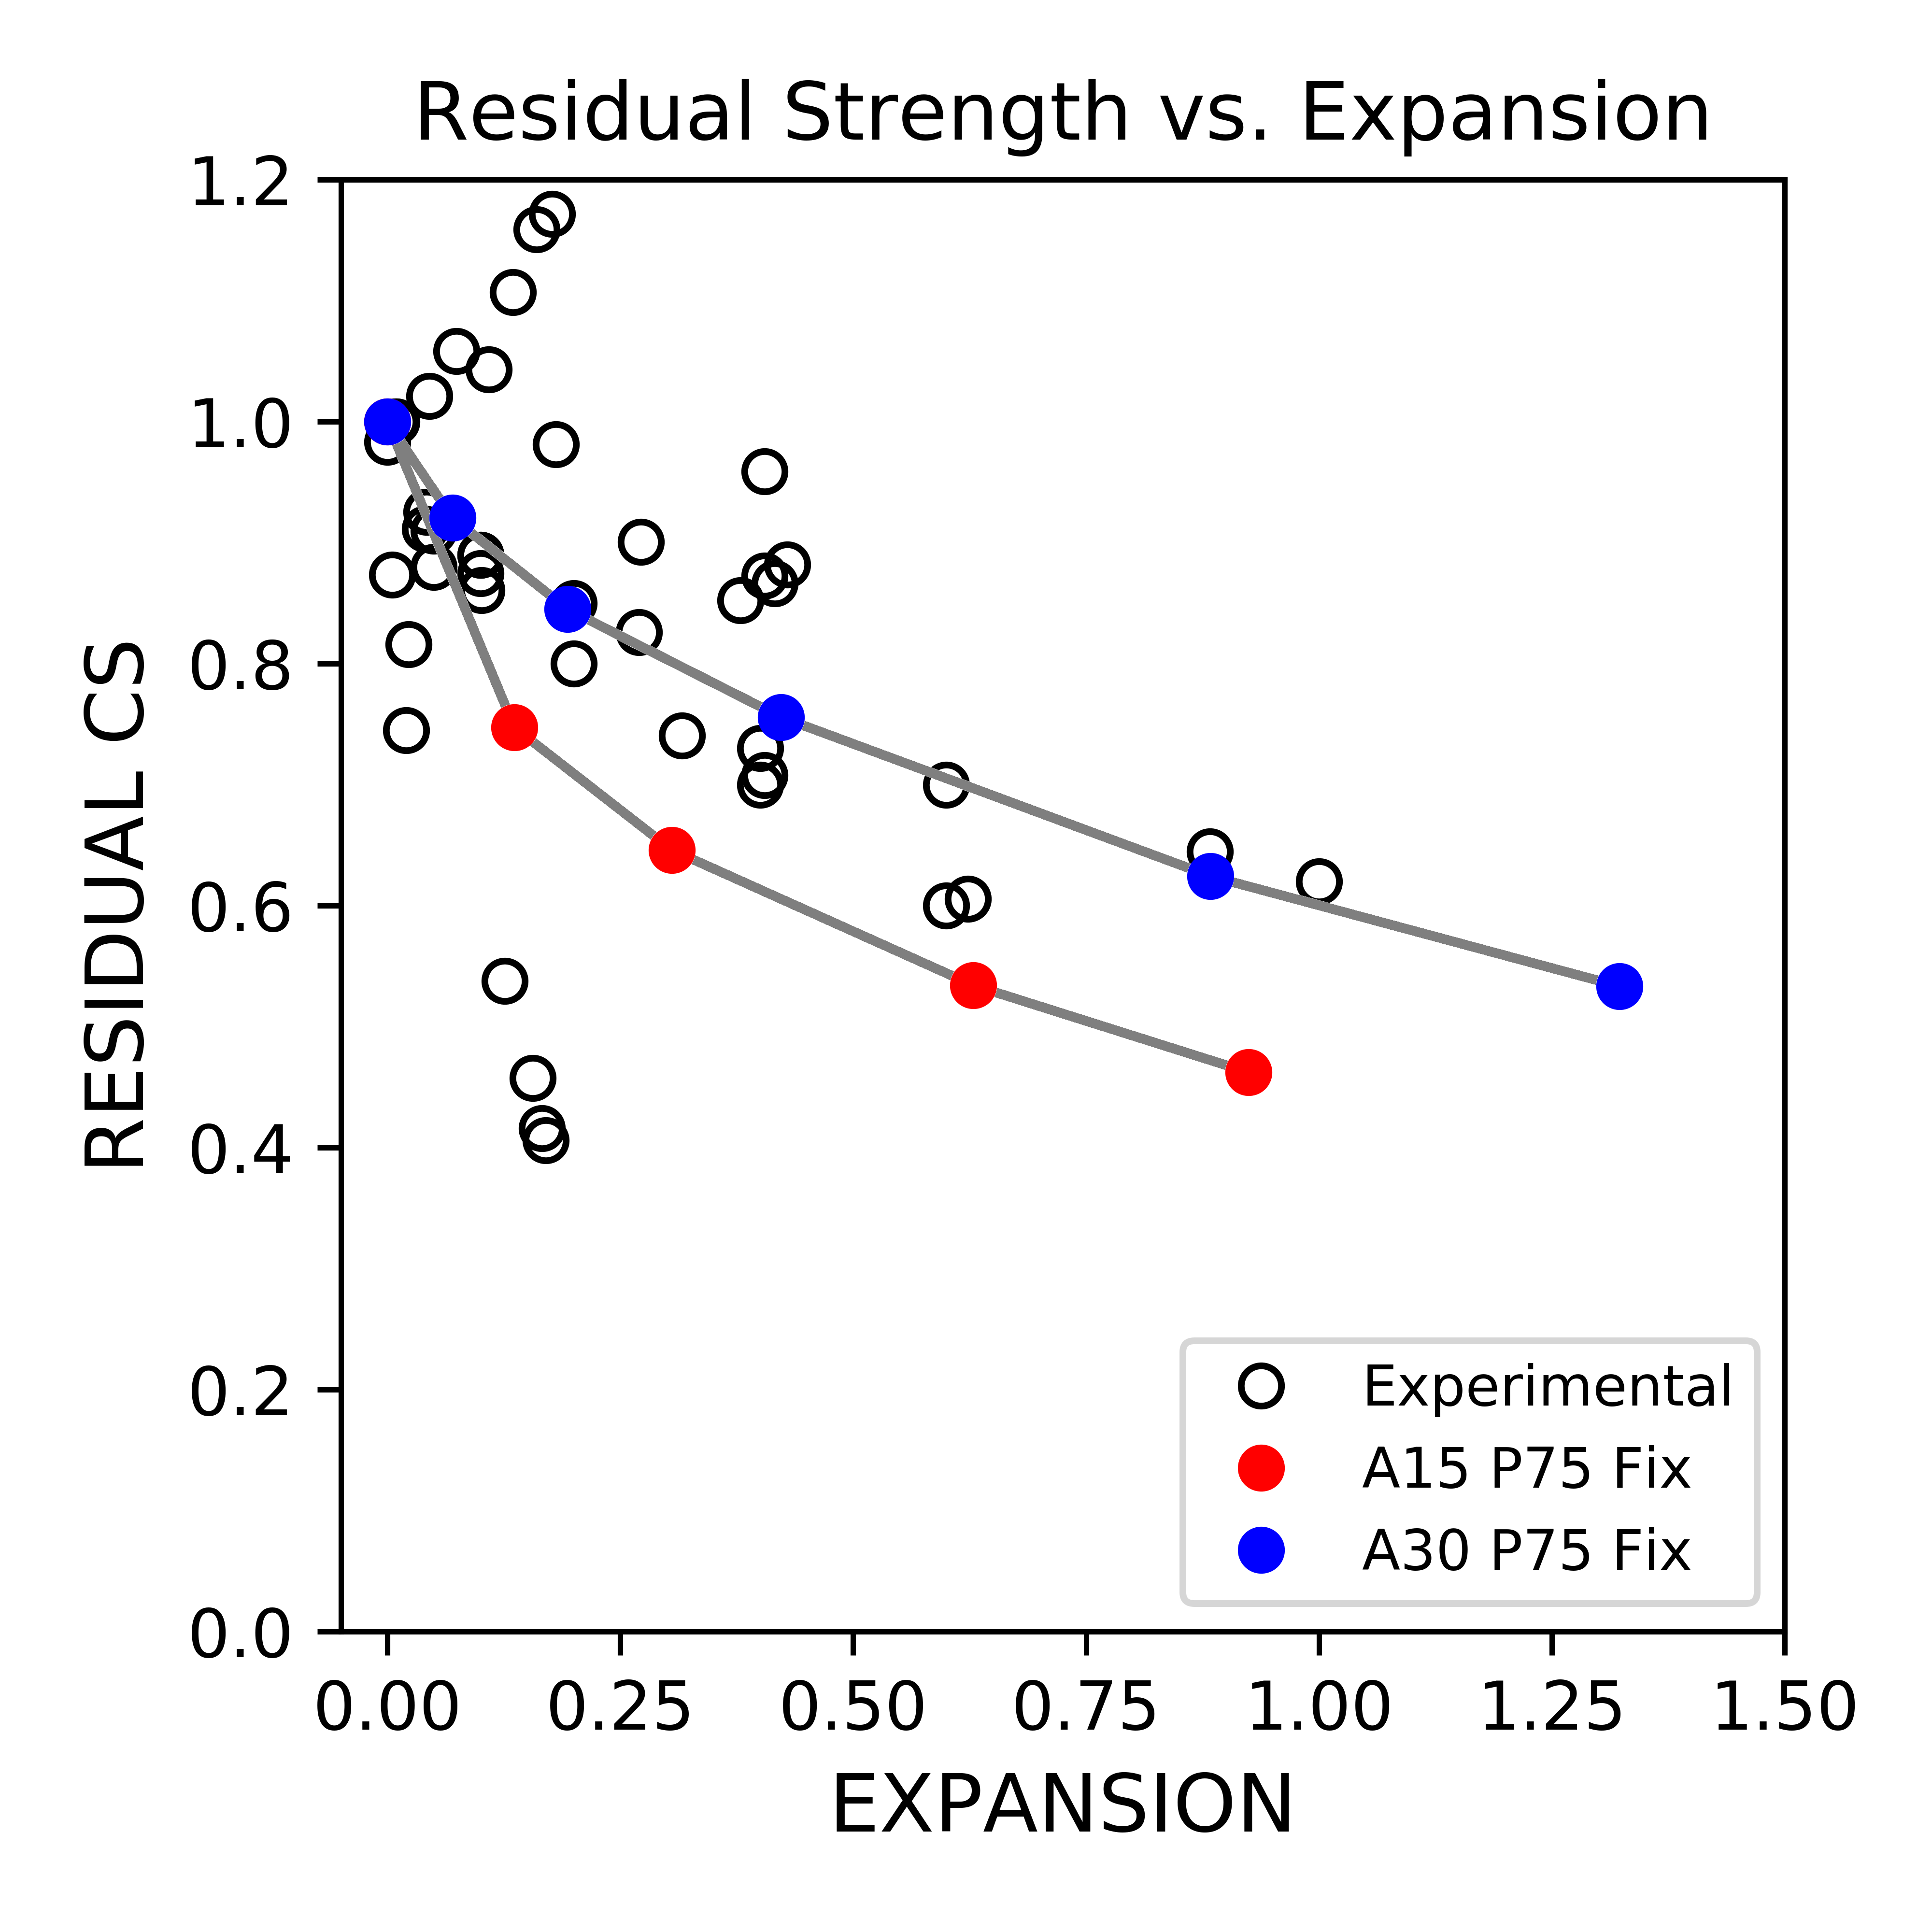
\includegraphics[width=.8\linewidth]{Files/CS_plot/ASRCS2.png}
  \caption{ASR Compressive Strength Comparing With Experimental Results}
  \label{ASRA30vsA15_cs}
\end{figure}

While in Figure \ref{A30P25vs75}, for the same 30\% coarse aggregate cases, if comparing 75\% ASR reactive aggregate results, which are labeled as A30 P75, and 25\% ASR reactive aggregate results, which are labeled as A30 P25, it can be seen that the residual compressive strength in 25\% ASR reactive aggregate cases are relative lower than the 75\% ASR reactive aggregate cases.

\begin{figure}[ht!]
\centering
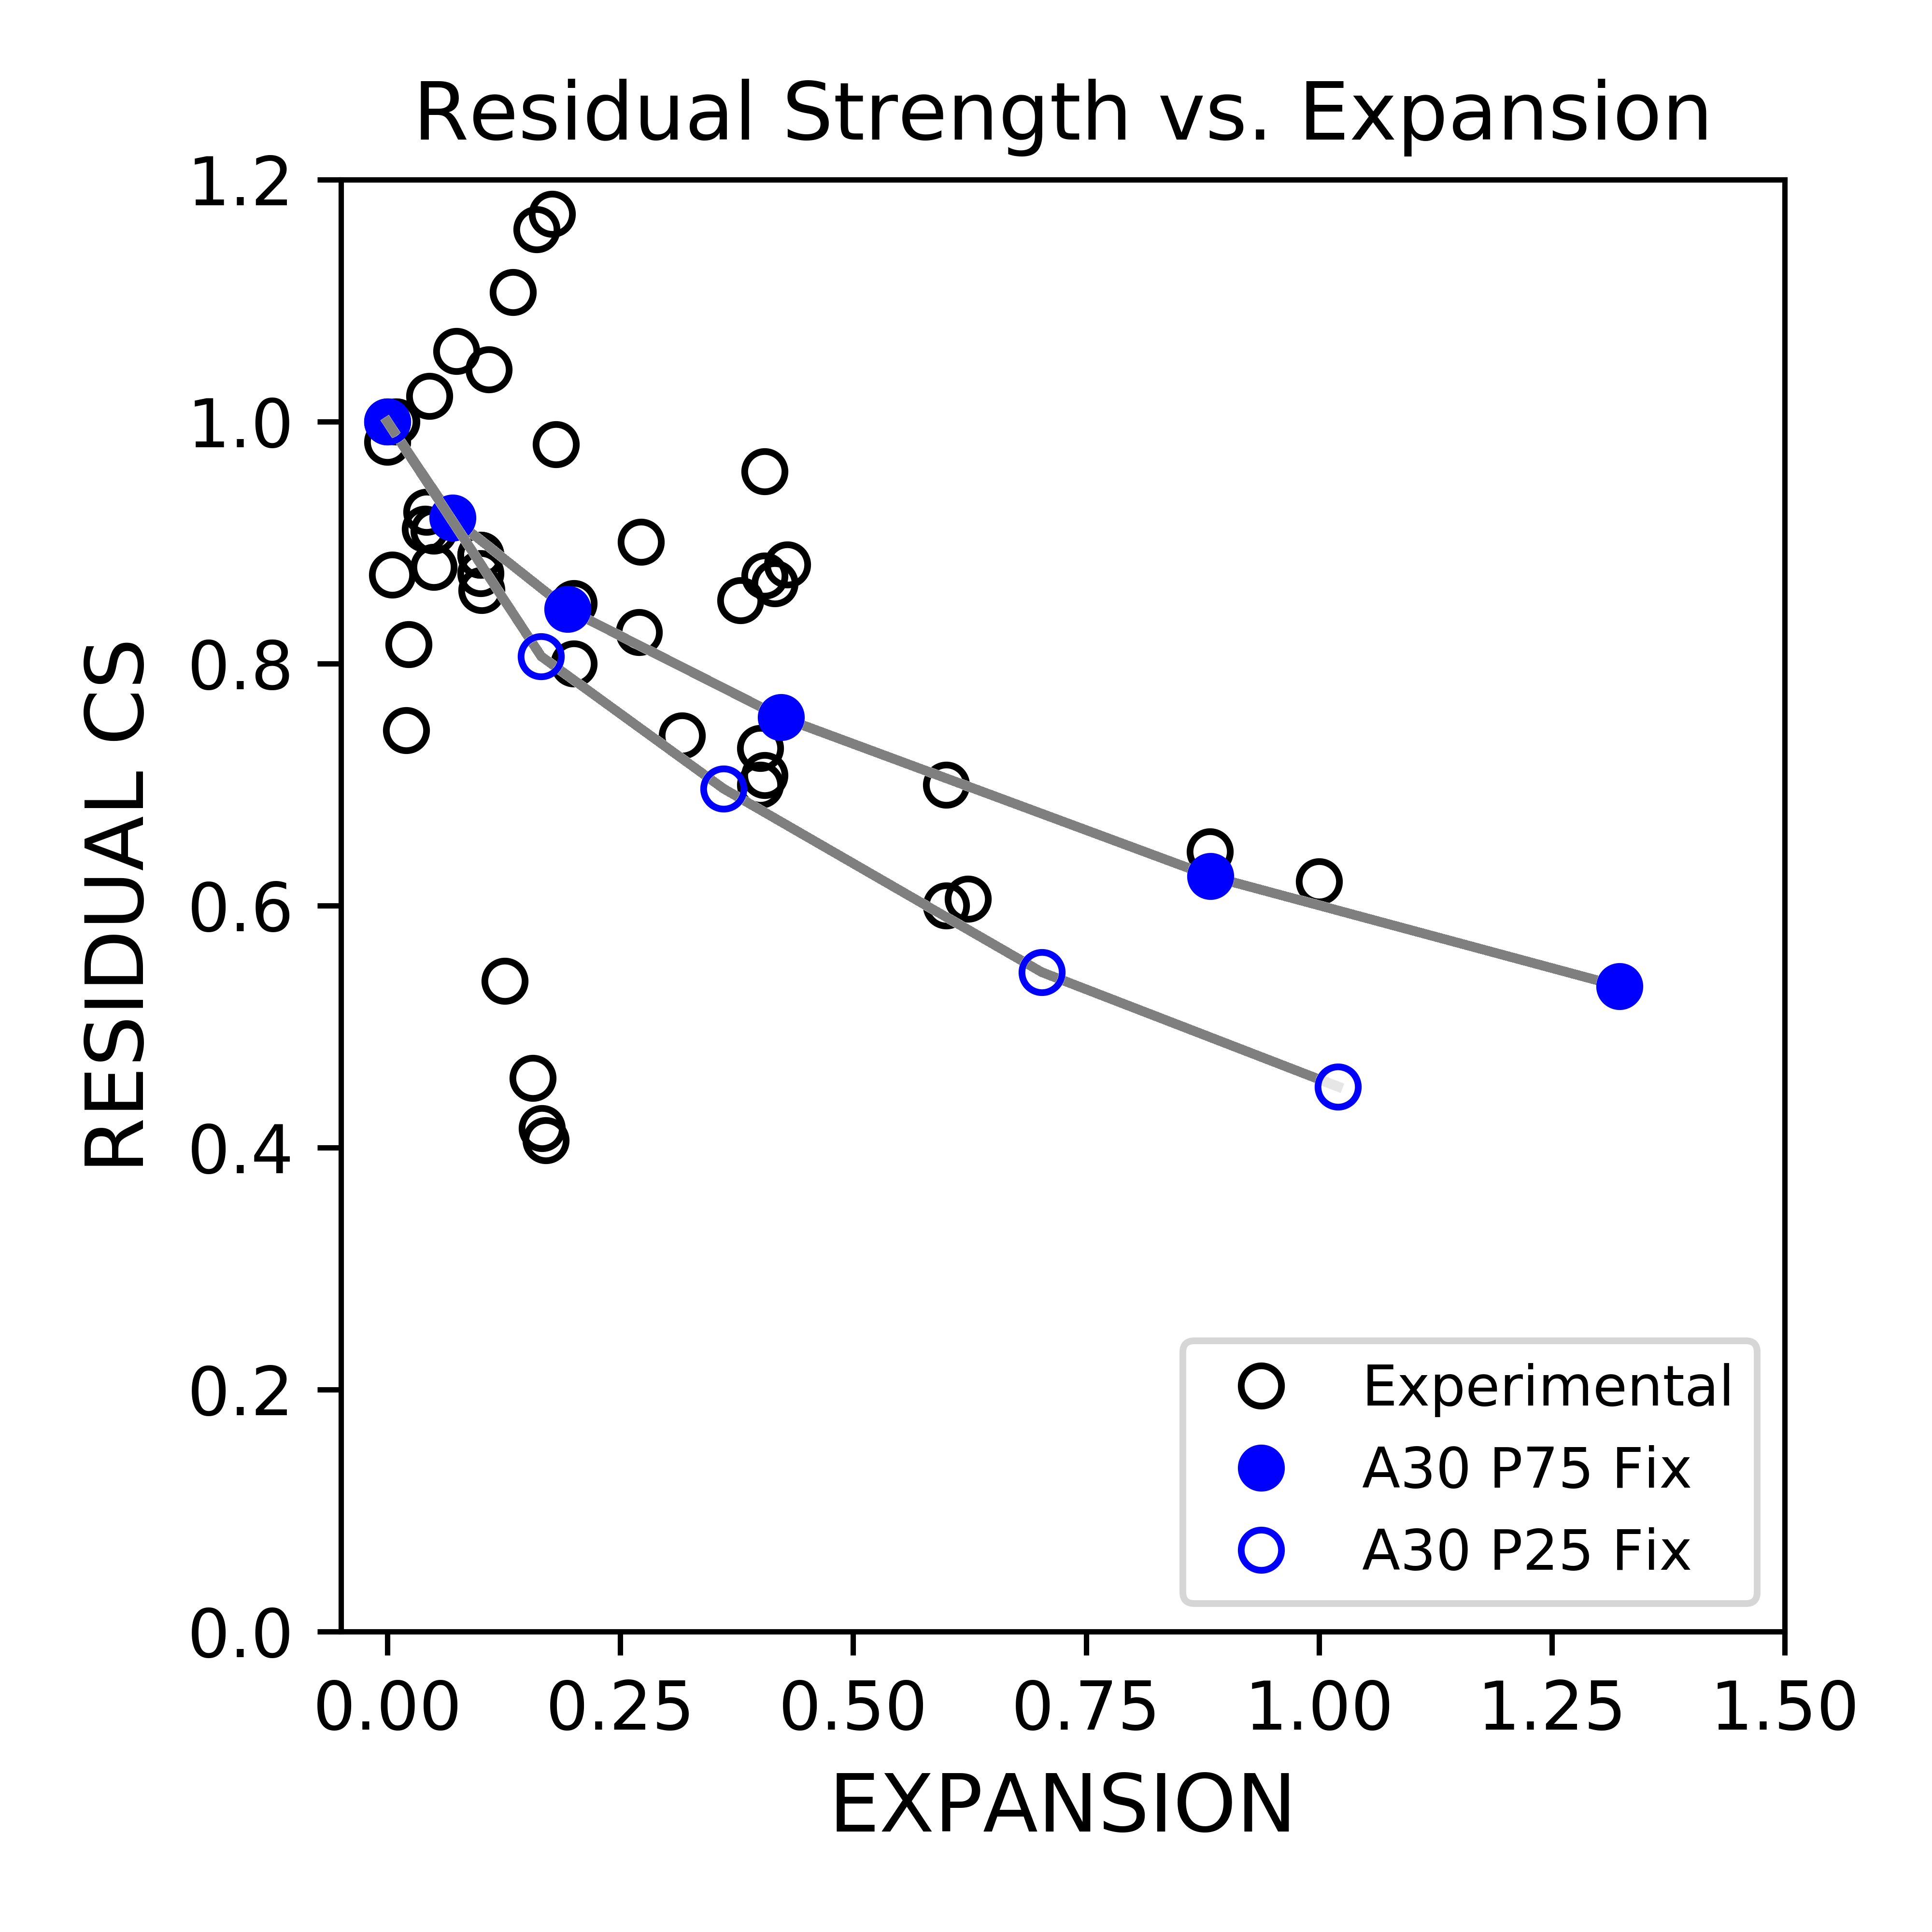
\includegraphics[width=.8\linewidth]{Files/CS_plot/ASRCS3.png}
  \caption{ASR Compressive Strength Comparing With Experimental Results}
  \label{A30P25vs75}
\end{figure}

These differences showing in different ASR expanding conditions implicated that the losses in mechanical properties are not only depends on the level of global expansion. In same amount of global expansion giving, the residual compressive strength can reach a difference up to around 30\%. Other factors also have impacts on concretes expanding behavior thus changing the mechanical properties of concrete. In later section, the relationship between cracking distribution in concrete model and its residual mechanical properties will be presented.

\begin{figure}[ht!]
\centering
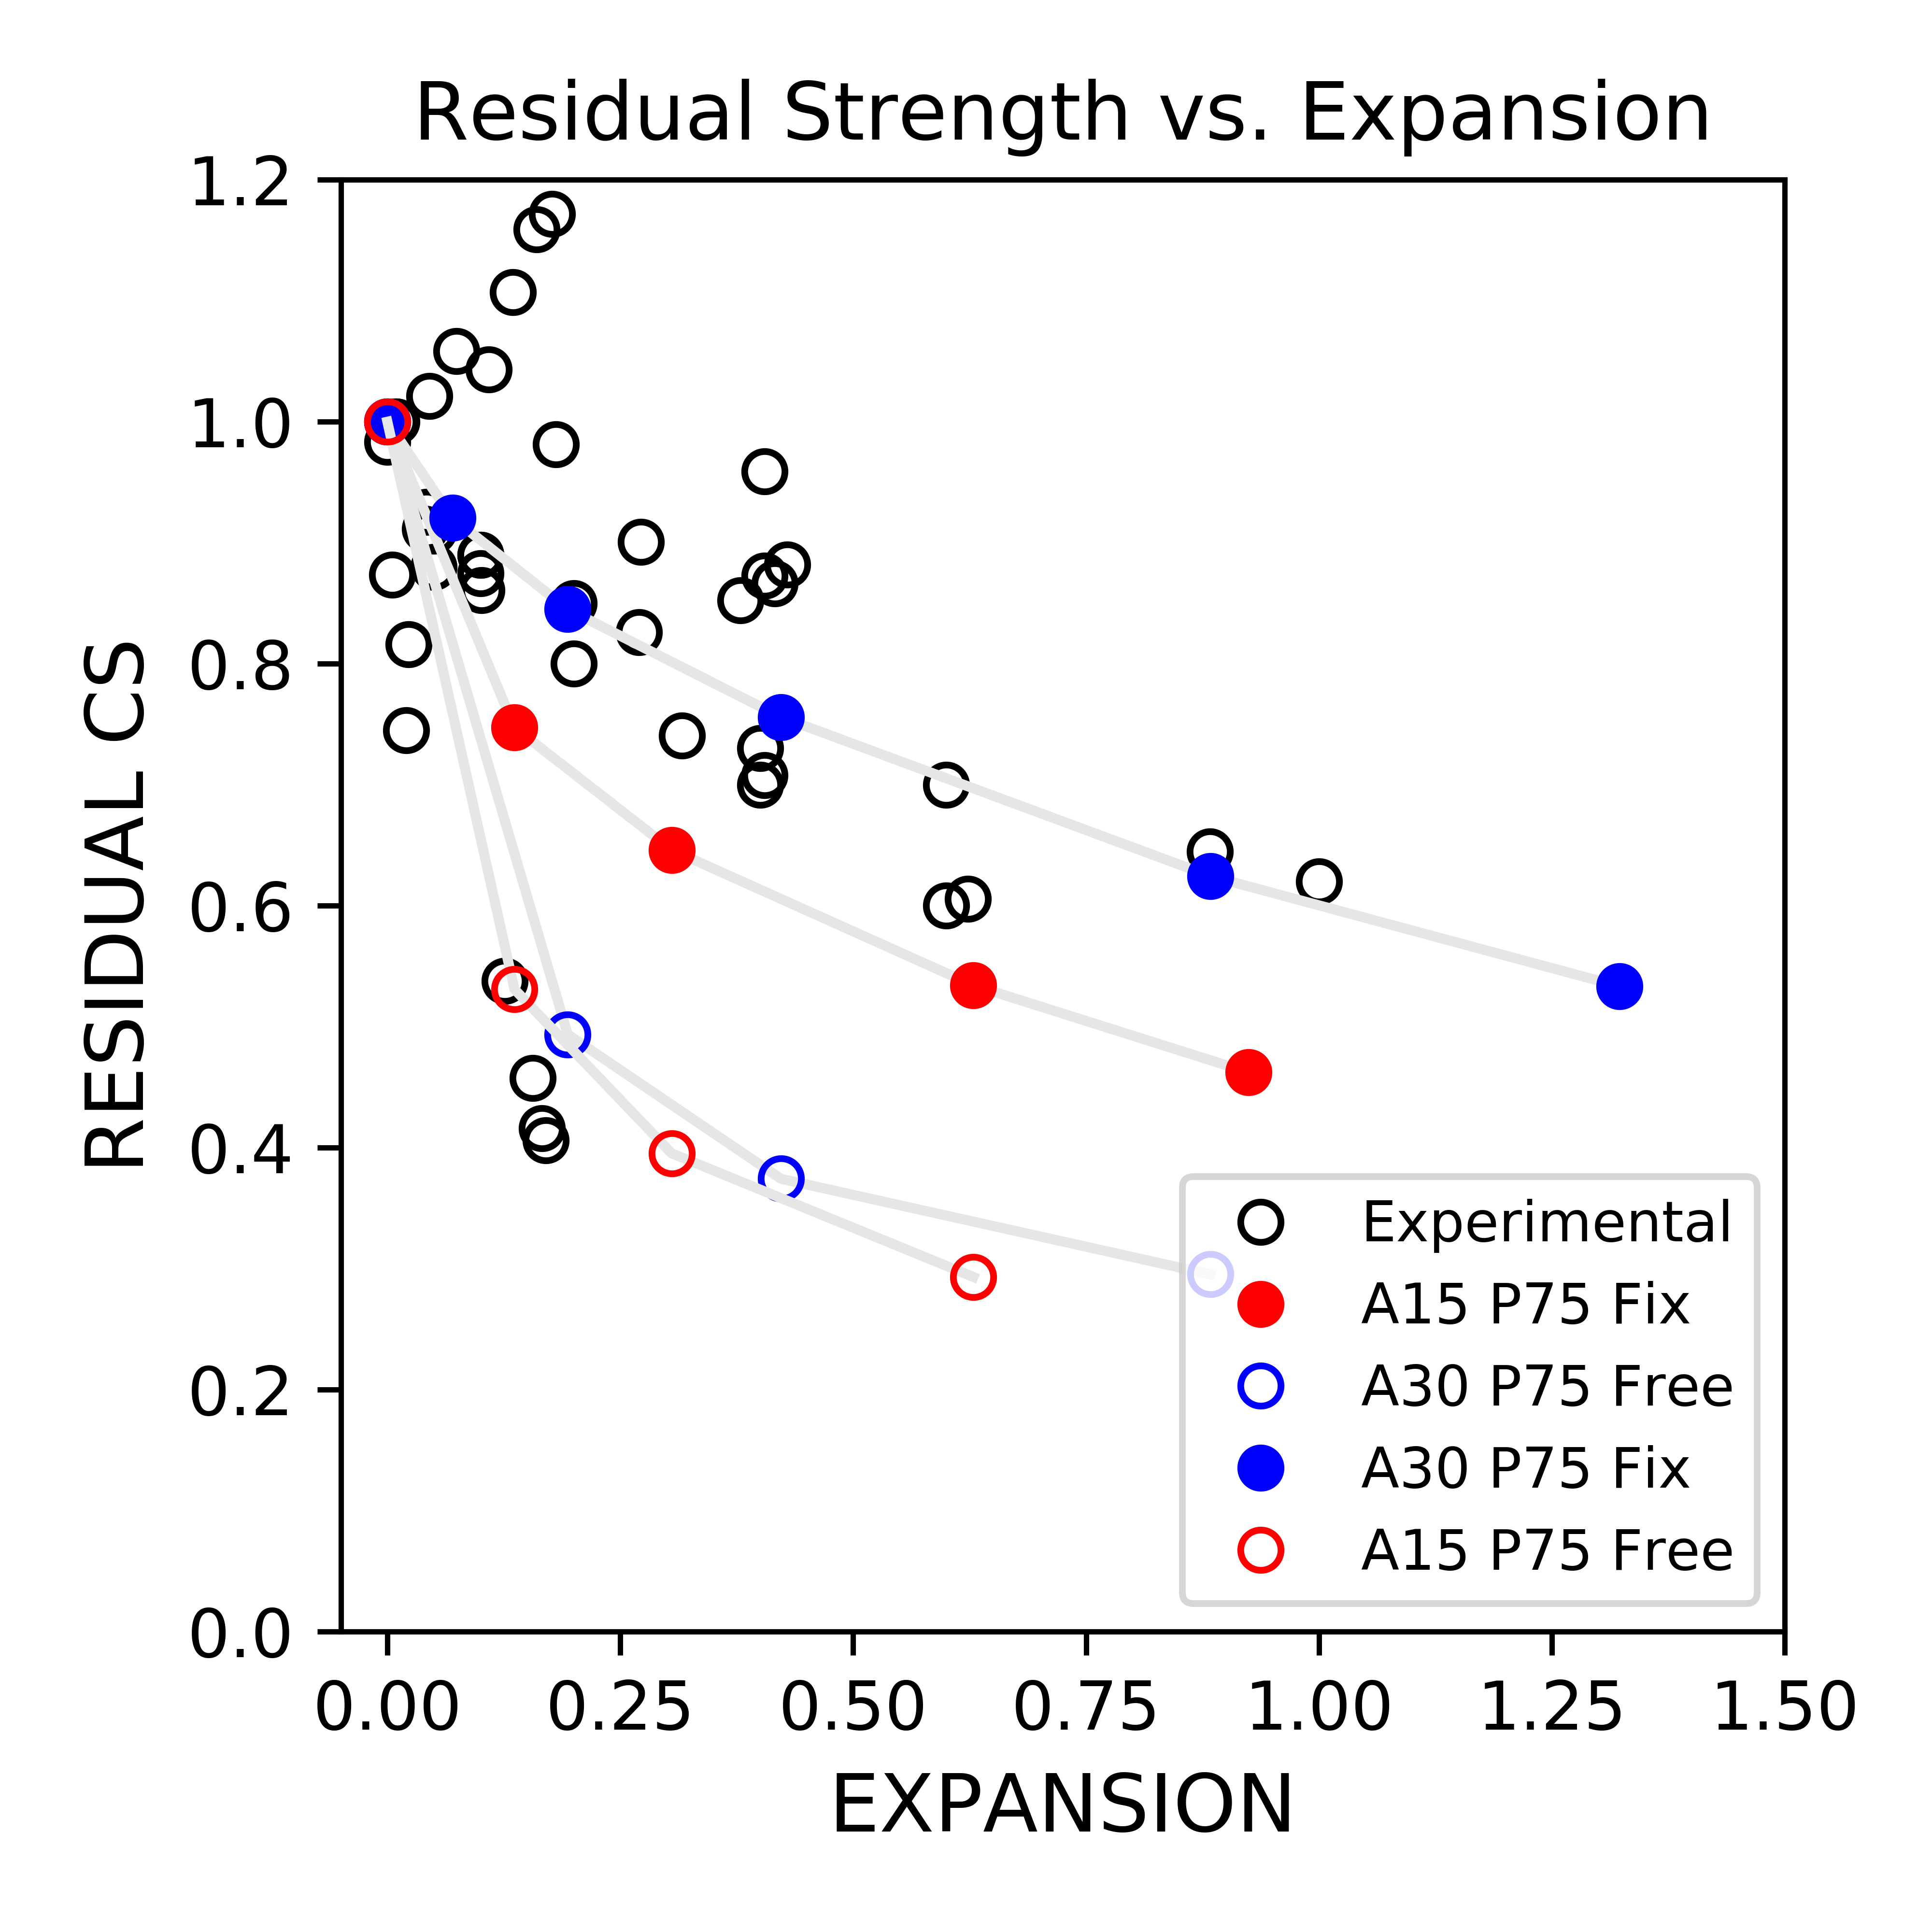
\includegraphics[width=.8\linewidth]{Files/CS_plot/ASR_free.png}
  \caption{ASR Compressive Strength Comparing With Experimental Results}
  \label{ASR_Free}
\end{figure}

Also, the free boundary condition is presented in Figure \ref{ASR_Free}, which shows relatively larger losses comparing to the fix boundary condition loading cases. This may due to the cracks generated from the expanding are much easier to open without restrain in the top and bottom boundary, causing larger losses in mechanical properties. However, the differences in residual compressive strength in differnt coarse aggregate percentage case are not significant in free boundary condition loading.
